\documentclass[upright, contnum]{umemoria}
\depto{DEPARTAMENTO DE CIENCIAS DE LA COMPUTACIÓN}
\author{Manuel Osvaldo J. Olguín Muñoz}
\title{Diseño e Implementación de un Framework Integrado para Simulaciones de Sistemas Inteligentes de Transporte en OMNeT++ y Paramics}
\auspicio{NIC Chile Research Labs y el Área de Transportes del Departamento de Ingeniería Civil de la Universidad de Chile}
\date{2017}
\guia{Sandra Céspedes Umaña}
\carrera{INGENIERO CIVIL EN COMPUTACIÓN}
\memoria{MEMORIA PARA OPTAR AL TÍTULO DE INGENIERO CIVIL EN COMPUTACIÓN}
\comision{Javier Bustos Jiménez, Nancy Hitschfeld Kahler}

\usepackage{lipsum}
\usepackage{multicol}
\usepackage[]{inputenc}
\usepackage[T1]{fontenc}
\usepackage{bytefield}
\usepackage{subcaption}
\usepackage{pgf-umlsd}
\usepackage{pgf-umlcd}
\usepackage[spanish]{babel}
\usepackage[style=ieee, sorting=none]{biblatex}
\usepackage{csquotes}
\usepackage{appendix}
\usepackage{listings}
\usepackage{float}
\usepackage{sourcecodepro}
\usepackage{tikz}
\usetikzlibrary{shapes.geometric, arrows}
\usepackage{tikz-qtree}
\usepackage{dirtree}
\usepackage[labelfont=bf]{caption}
\usepackage{enumitem}
\usepackage{hyperref}
\usepackage[htt]{hyphenat}

\inputencoding{utf8}

\renewcommand{\labelenumii}{\roman{enumii}.}

\setlist{  
    listparindent=\parindent
}

% reference description items
\makeatletter
\def\namedlabel#1#2{\begingroup
    #2%
    \def\@currentlabel{#2}%
    \phantomsection\label{#1}\endgroup
}
\makeatother

\captionsetup{format=hang}

% CPP style definition: %
\renewcommand{\lstlistingname}{Código}% Listing -> Código
\renewcommand{\lstlistlistingname}{Lista de \lstlistingname s}% List of Listings -> List of Algorithms
\definecolor{dkgreen}{rgb}{0,0.6,0}
\definecolor{gray}{rgb}{0.5,0.5,0.5}
\definecolor{lightgray}{rgb}{0.95, 0.95, 0.95}
\definecolor{mauve}{rgb}{0.58,0,0.82}
\definecolor{mygreen}{rgb}{0,0.6,0}
\definecolor{mygray}{rgb}{0.5,0.5,0.5}
\definecolor{mymauve}{rgb}{0.58,0,0.82}
\lstdefinestyle{CPP}{ % Estilo de lenguaje C++11
    language=[11]C++,
    frame=Lbtr,
    xleftmargin=\parindent,
    captionpos=b,
    aboveskip=3mm,
    belowskip=3mm,
    showstringspaces=false,
    columns=flexible,
    basicstyle={\small\ttfamily},
    numbers=left,
    numberstyle=\tiny\color{gray},
    keywordstyle=\color{purple},
    commentstyle=\color{gray},
    stringstyle=\color{dkgreen},
    breaklines=true,
    breakatwhitespace=true,
    tabsize=4,
    morekeywords={string,define,\#},
    otherkeywords={\#},
    backgroundcolor=\color{lightgray},
    escapeinside={/l*}{*l/}
}

\lstdefinestyle{myXML}{ % Estilo de lenguaje C++11
    language=XML,
    frame=Lbtr,
    xleftmargin=\parindent,
    captionpos=b,
    aboveskip=3mm,
    belowskip=3mm,
    showstringspaces=false,
    columns=flexible,
    basicstyle={\small\ttfamily},
    numbers=left,
    numberstyle=\tiny\color{gray},
    keywordstyle=\color{purple},
    commentstyle=\color{gray},
    stringstyle=\color{dkgreen},
    breaklines=true,
    breakatwhitespace=true,
    tabsize=4,
    morekeywords={xml,version, launch, basedir, network, seed},
    otherkeywords={\#},
    backgroundcolor=\color{lightgray},
    escapeinside={/l*}{*l/}
}

\lstdefinestyle{MyPython}{ % Estilo de lenguaje C++11
    language=Python,
    frame=Lbtr,
    xleftmargin=\parindent,
    captionpos=b,
    aboveskip=3mm,
    belowskip=3mm,
    showstringspaces=false,
    columns=flexible,
    basicstyle={\small\ttfamily},
    numbers=left,
    numberstyle=\tiny\color{gray},
    keywordstyle=\color{purple},
    commentstyle=\color{gray},
    stringstyle=\color{dkgreen},
    breaklines=true,
    breakatwhitespace=true,
    tabsize=4,
    morekeywords={traci, print},
    otherkeywords={},
    backgroundcolor=\color{lightgray},
    escapeinside={/l*}{*l/}
}

% new an instance thread
% Example:
% \newthread[edge distance]{var}{thread name}
\renewcommand{\newthread}[3][0.2]{
    \newinst[#1]{#2}{#3}
    \stepcounter{threadnum}
    \node[below of=inst\theinstnum,node distance=0.8cm] (thread\thethreadnum) {};
    \tikzstyle{threadcolor\thethreadnum}=[fill=gray!30]
    \tikzstyle{instcolor#2}=[fill=gray!30]
}

\newcommand{\blankpage}{
    \newpage
    %\thispagestyle{empty}
    \mbox{}
    \newpage
}

\newcommand{\minipagelisting}[3]{
    \noindent
    \begin{minipage}{\linewidth}
        \lstinputlisting[style=CPP, label={#3}, caption={#2}]{#1}
    \end{minipage}
}

\newcommand\mcitem[1]{\item\begin{minipage}[t]{\linewidth}#1\end{minipage}}

% footnote spacing
\setlength{\footnotesep}{.7cm}
\addbibresource{bibliografia.bib}


\begin{document}

\frontmatter
\maketitle

\date{Junio 2017}
\begin{abstract}
El presente trabajo de memoria presenta el diseño, implementación y validación de un \emph{framework} de integración de un simulador de transporte, \emph{Quadstone Paramics} con un simulador de redes comunicaciones inalámbricas, \emph{OMNeT++}, para la simulación y estudio de Sistemas Inteligentes de Transporte.

Los Sistemas Inteligentes de Transporte surgen como una respuesta a la necesidad de optimización, modernización y mejoramiento de los actuales sistemas de transporte. Los Sistemas de Transporte Inteligente pretenden proveer servicios innovadores que otorguen información a los usuarios y les permitan utilizar el sistema de transporte de manera más segura, coordinada e inteligente. Resulta fundamental la recopilación y transmisión de información en estos sistemas, lo cual se realiza mediante implementación de redes comunicación inalámbrica, tanto entre vehículos como entre vehículos e infrestructura. Es necesario entonces el desarrollo de entornos de software de modelamiento y simulación de estos sistemas, para su estudio previo a su implementación en el mundo real.

Este trabajo de memoria presenta un \emph{framework} que posibilita la simulación y análisis de los Sistemas Inteligentes de Transporte. PVEINS, como se denomina el software desarrollado, permite el estudio de la integración bidireccional de un sistema de transporte con un sistema de comunicaciones inalámbricas. En ese sentido, el \emph{framework} permite determinar tanto el impacto de la comunicación entre vehículos sobre el modelo de transporte, como el impacto del movimiento de los vehículos sobre el medio de comunicación entre estos.

El software consiste principalmente en un \emph{plugin} para Paramics, escrito en C++, el cual permite la integración transparente de este simulador con un \emph{framework} de simulación de Sistemas Inteligentes de Transporte ya existente y de gran renombre en la academia. Se desarrolló utilizando una estrategia iterativa, siguiendo buenas prácticas de ingeniería de software.

Finalmente, el presente trabajo de memoria presenta además un análisis de eficiencia del software desarrollado, y un estudio para verificar su validez para la simulación de sistemas de transporte de alta complejidad. Los resultados son altamente positivos, y demuestran que PVEINS tiene el potencial para posicionarse como una opción competitiva para la simulación de Sistemas Inteligentes de Transporte en la academia.
\end{abstract}

\begin{dedicatoria}
Den här är för Aros och Skatt,\\ som alltid stöttat mig\\ ovillkorligt som bara hundar kan.
\end{dedicatoria}

\begin{thanks}
    Son muchos, tal vez demasiados, a quienes debo agradecer por su apoyo, amistad y/o cariño en el camino al obtener mi título. 
    
    En primer lugar, quiero agradecer a mi familia, quienes siempre han estado presentes y me inculcaron desde el primer momento el valor del estudio y el esfuerzo. 
    A mi padre, Gabriel Olguín, por ser mi ejemplo a seguir en el ámbito académico - me lleva un doctorado y un postdoc de ventaja, pero eventualmente lo alcanzaré. 
    A mi madre, Valeria Muñoz, por ser una constante de estabilidad emocional en mi vida y que también desde siempre me ha impulsado a alcanzar las estrellas. Me ha tenido que soportar 24 años, pero finalmente llegó este mi primer paso en mi independización.
    A mi hermana, Paola Olguín, por soportar mis estupideces todos los días -- me llena de orgullo saber que ella sigue mis pasos y que se dedicará a la misma carrera que yo. Y a mis abuelos, quienes siempre me han dado apoyo incondicional. 
    En especial, a mi Tata Caupolicán Muñoz, con quien siempre compartí profundas discusiones sobre ciencia y quien me inculcó el amor por la lectura. Yo sé que estaría hinchado de orgullo al verme recibirme de ingeniero civil.
    
    También quiero darle mis profundas gracias a los profesores que me han acompañado en este largo proceso. 
    A la profesora Sandra Céspedes, por ser probablemente la mejor profesora guía que podría haber pedido -- le pido disculpas por todos esos correos y mensajes en fines de semana, que ella respondió de manera muy cordial.
    A Javier Bustos, por haberme dado la oportunidad en su momento de realizar mi práctica en NICLabs a pesar de que no tenía las mejores calificaciones, y por haberme aceptado más tarde como miembro permanente del equipo. Espero haberle demostrado que tomó la decisión correcta.   
    A Cristián Cortés, por su invaluable apoyo durante mi trabajo de memoria, y tremendo entusiasmo con los resultados que le he presentado.
    A la profesora Nancy Hitschfeld, quien fue la primera en confiar en mis habilidades para enseñar, y me aceptó como profesor auxiliar en su curso de computación gráfica. Me abrió el mundo de la docencia, el cual me fascinó y por lo cual le estoy eternamente agradecido.
    Al profesor Jérémy Barbay, por haber sido tanto un tutor como un amigo en estos años -- gracias por los infinitos consejos, los buenos momentos y la oportunidad de desarrollar algo tan novedoso como lo fue Moulinette. 
    
    A mis amigos, quienes me han soportado durante todos estos años, en las buenas y en las malas, gracias. 
    En especial quiero nombrar a mis amigos más cercanos de éstos últimos años; JP, Juanjo, Negro y Varas -- gracias amigos por haberme apoyado cuando necesitaba apoyo, haberme corregido cuando necesitaba ser corregido y por haberme insultado cuando necesitaba ser insultado. 
    Un abrazo también para los chiquillos del ``\emph{lolcito}''; Diego, George y el resto del equipo -- no sé que hubiese hecho estos años sin esas partidas nocturnas que me alejaban del estrés diario de los estudios. 
    Quiero además agradecer a mi polola, Maria Collin, por su paciencia y su enorme corazón -- su cariño y apoyo me han impulsado a trabajar más duro que nunca.
    
    \emph{Last, but not least,} como dicen en inglés, quiero agradecer a todo el resto del mundo que no cupo en los párrafos anteriores -- no me he olvidado de ustedes. 
    Gracias por el apoyo, las palábras de ánimo, la buena onda. 
    A todos, de todo mi corazón: a mis amigos del colegio, a mis amigos de la universidad, a los profesores del gimnasio, al tío del kiosko a quien semana tras semana le compré bebidas energéticas para seguir adelante. 
    Gracias!\\
    
    \begin{flushright}
        \textit{Manuel Osvaldo J. Olguín Muñoz}
    \end{flushright}
\end{thanks}

%\cleardoublepage
\tableofcontents
%\cleardoublepage
\listoftables
%\cleardoublepage
\listoffigures

\mainmatter

\chapter{Introducción}
\section{Motivación}

Los sistemas de transporte conforman la columna vertebral de nuestras ciudades, contribuyendo directamente al desarrollo de la sociedad urbana. Un sistema de transporte bien diseñado y eficiente permite el desplazamiento rápido y cómodo de personas y bienes; en cambio, uno ineficiente genera grandes problemas, alargando los tiempos de viaje y aumentando la contaminación atmosférica.

Los Sistemas de Transporte Inteligente surgen como una respuesta a la necesidad de optimización, modernización y mejoramiento de los sistemas de transporte ya existentes. La Unión Europea define a los ITS como aplicaciones que pretenden proveer servicios innovadores relacionados con distintos modos de transporte y de administración de tráfico, que además otorgan información a los usuarios y les permiten utilizar el sistema de transporte de manera más segura, coordinada e inteligente \cite{eudirective}. Esta amplia definición abarca una gran cantidad de aplicaciones: desde sistemas de alerta temprana a sistemas de entretención en ruta, pasando incluso por aplicaciones tan avanzadas como sistemas de coordinación y control de vehículos autónomos.

%\begin{figure}[tpb]
%    \centering
%    \includegraphics[width=0.9\linewidth]{figuras/ITS.png}
%    \caption{Aplicaciones en un Sistema Inteligente de Transporte (fuente: ETSI \autocite{etsi}).}
%    \label{fig:itsetsi}
%\end{figure}

El factor común entre todas estas aplicaciones es la necesidad de extraer información en tiempo real desde el entorno, la cual debe procesarse y en muchos casos generar una respuesta a transmitir al usuario. Para este fin, se ha propuesto la implementación de tecnologías que posibiliten esta comunicación, principalmente utilizando redes inalámbricas, tanto de área local (los estándares incluídos en la familia WLAN, IEEE 802.11), como de área personal (WPAN, IEEE 802.15) \cite{80211dailey,80215vanet,80211wave}. Sin embargo, estas tecnologías fueron diseñadas originalmente para su uso en redes estáticas o con patrones de movimiento muy limitados, y es necesaria la evaluación de su desempeño en entornos altamente dinámicos como lo son los sistemas de transporte vehicular. Parámetros críticos para el funcionamiento óptimo de la red, como la potencia de transmisión, las condiciones del canal de transmisión y la distancia óptima entre nodos, deben establecerse teniendo en cuenta las particularidades que presentan los sistemas de transporte -- por ejemplo, la alta congestión de nodos en intersecciones con semáforos.

Existe entonces hoy en día la necesidad de modelar de manera realista y precisa el comportamiento de estas tecnologías en contextos de comunicaciones inalámbricas en redes vehiculares. Por otro lado, existe también la necesidad de modelar el impacto de la comunicación inalámbrica en un sistema de transporte, y cómo esta puede contribuir a optimizar la operación del mismo \cite{sommer2008need, bidirectionalsimul}. Un ejemplo de esto son los Sistemas Avanzados de Información al Viajero (\textit{ATIS}, por sus siglas en inglés; \textit{Advanced Traveller Information System}) los cuales proveen información en tiempo real sobre las condiciones del tránsito a conductores, permitiéndoles elegir la ruta más óptima para alcanzar su destino. Este \textit{feedback} inmediato sin duda tiene efectos importantes en el flujo vehicular de un sistema de transportes, los cuales deben ser tomados en consideración al momento de modelar y simular el funcionamiento del mismo.
\section{Resumen}

A raíz de la problemática expuesta en la sección anterior, el presente trabajo de memoria presenta un \emph{framework} de integración bidireccional entre un simulador de redes de comunicaciones inalámbricas -- OMNeT++ -- con un simulador de redes de transporte -- Quadstone Paramics -- como una herramienta de apoyo para el estudio de las problemáticas previamente señaladas y la evaluación de nuevos modelos y soluciones para transporte inteligente.

La elección de éstos simuladores en particular tiene razones bien fundadas. En particular, OMNeT++ fue escogido principalmente por particularidades que se verán más adelante, relacionadas con la elección de solución al problema planteado. Por otro lado, Paramics es el simulador de transporte de preferencia del Departamento de Transportes de la Universidad de Chile, parte interesada en el presente proyecto de memoria dadas las aplicaciones que puede tener para la investigación que se realiza en el Departamento. La extensión de Paramics para su funcionamiento en un sistema de simulación integrado bidireccional permitiría a su vez la extensión de modelos ya existentes que maneja dicha área de investigación, para sus estudios en contextos de Sistemas de Transporte Inteligente.

El \emph{framework} desarrollado para la memoria se implementó en base a una adaptación de un trabajo previamente realizado por Sommer \emph{et al.} \autocite{sommer_german_dressler, sommer_dressler2} para la integración de OMNeT++ con SUMO, otro simulador de redes de transporte. Este trabajo previo, un \emph{framework} denominado VEINS -- por sus siglas en inglés, \emph{Vehicles In Network Simulation} -- utiliza una novedosa arquitectura en la que ambos simuladores se comunican a través de un \emph{socket}, en una configuración cliente-servidor. La implementación presentada en este trabajo de memoria, denominada PVEINS\footnote{PVEINS -- \textbf{P}aramics \textbf{VEINS}}, pretende reemplazar, de manera absolutamente transparente para OMNeT++, a SUMO en dicha arquitectura, para así poder aprovechar todo el trabajo en modelos de comunicación ya existentes para esta configuración.

\begin{figure}[tpb]
    \centering
    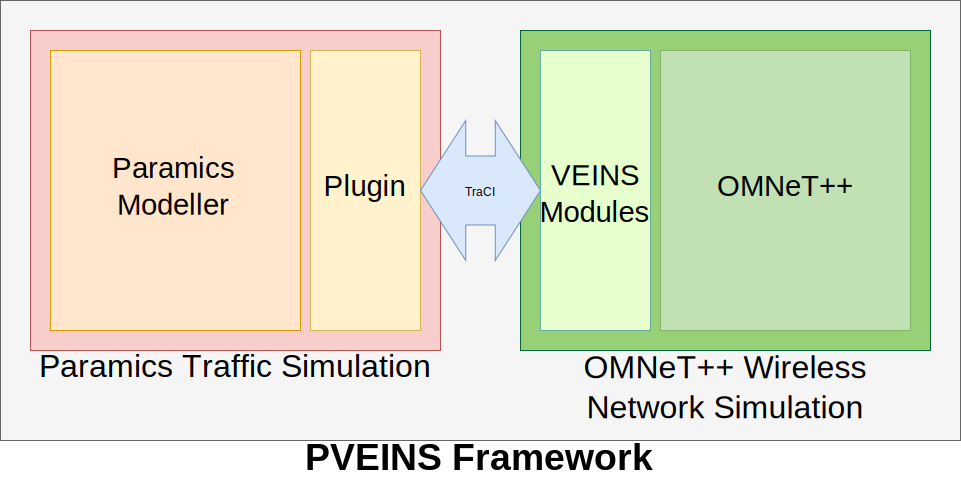
\includegraphics[width=\linewidth]{figuras/PVEINSArch.png}
    \caption{Integración bidireccional de Paramics con OMNeT++.}
    \label{fig:pveins_genarch:resumen}
\end{figure}

El trabajo consistió principalmente en el desarrollo de un \emph{plugin} de extensión de Paramics, el cual se encarga de recibir e interpretar comandos desde el simulador de redes, realizando las operaciones necesarias en el modelo de Paramics. Este se desarrolló en C++, en su estándar 2011, utilizando la API del software (ver apéndice \ref{anex:paramics_api}).

Este \emph{plugin} permite la integración de Paramics con el entorno de simulación de OMNeT++, posibilitando la simulación de Sistemas Inteligentes de Transporte -- el \emph{framework} permite al simulador de redes construir una red inalámbrica equivalente a la red de transporte simulada, donde cada vehículo en Paramics se asocia a un nodo dotado de capacidades de comunicación inalámbrica en OMNeT++. El estado de ambas simulaciones evoluciona de manera sincronizada, y los nodos de OMNeT++ están dotados de lógica y pueden modificar el comportamiento de sus respectivos vehículos. De esta manera, es posible analizar tanto el impacto de la movilidad de los vehículos sobre el canal de comunicaciones, como el impacto de la transmisión de información en el modelo de transporte.

Este nuevo \emph{framework} PVEINS se validó luego mediante una serie de experimentos destinados a medir su rendimiento y su aptitud para uso en investigación y modelación de Sistemas Inteligentes de Transporte de una complejidad considerable. El Área de Transportes del Departamento de Ingeniería Civil de la Universidad de Chile proporcionó un escenario realista que modela un sector de la ciudad de Santiago en hora punta, el cual se utilizó para la validación del \emph{software}. Este escenario es de alta complejidad, elaborado por Zúñiga \autocite{zuniga} en 2010 para su memoria de título, y presenta un promedio de aprox. 1400 vehículos presentes en la red en cada instante de la simulación. 

Los resultados de los análisis realizados sobre el \emph{framework} en el contexto de un escenario tan complejo como el proporcionado fueron altamente positivos. El software es eficiente, y permite modelar de manera precisa y realista el comportamiento de los Sistemas Inteligentes de Transporte.

Sin embargo, este trabajo de todas maneras identifica factores y detalles perfeccionables en la implementación del sistema, los cuales se presentan al final de este documento como sugerencias para trabajo futuro. 

Finalmente, el producto de este trabajo de memoria se encuentra disponible en su totalidad en el repositorio \emph{git} personal del autor \autocite{pveins_github}, bajo una licencia \emph{BSD 3-Clause} \autocite{bsd3clause}. Ahí se podrá encontrar tanto el código fuente del \emph{framework} como del escenario de validación avanzado y los resultados de las pruebas realizadas.
\section{Organización del documento}

El presente documento de memoria se estructura como sigue; el presente capítulo expone la motivación tras el proyecto desarrollado, y los objetivos principales que se pretendían lograr con la implementación de éste. 

El capítulo \ref{cap:marcoteo} expone el marco téorico que sustenta el trabajo de memoria, además de presentar una extensa revisión del estado del arte en los ámbitos de simulación de sistemas de transporte, de redes de comunicaciones y de simulación bidireccional entre las dos categorías anteriores.

A continuación, en el capítulo \ref{cap:diseno} se detallan las decisiones de diseño macroscópico que se tomaron al elaborar la arquitectura del proyecto, y las evoluciones por las cuales este diseño pasó. Se presenta además la metodología de trabajo utilizada para el desarrollo del \emph{software} y las funcionalidades implementadas en términos generales.

En el capítulo \ref{cap:implementation} Implementación, se describe en detalle la implementación en código del \emph{framework}, además de entregarse una breve descripción de las pruebas que se realizaron durante el desarrollo.

El capítulo siguiente, el capítulo \ref{cap:validacion}, expone el escenario avanzado de prueba que se utilizó para evaluar el rendimiento y la efectividad del proyecto. Se presentan además los resultados obtenidos de las pruebas realizadas, y se realiza un análisis de éstos.

Finalmente, el capítulo \ref{cap:conclusion} concluye la presente memoria, realizando un análisis general de los resultados obtenidos, verificando que se cumplieron los objetivos establecidos en la sección \ref{sec:obj} y presentando trabajo futuro a realizar.



\chapter{Marco Teórico y Estado del Arte}
\section{Marco Teórico}

En esta sección se detallarán los conceptos esenciales para la comprensión del presente trabajo de memoria.

\subsection{Sistemas de Transporte}

Cascetta define en \autocite{cascetta2013transportation} a los sistemas de transporte como aquella combinación de elementos que generan demanda de viaje en un cierta área geográfica, y que otorgan los servicios de transporte para suplir dicha demanda. Esta definición es amplia y otorga una visión general del concepto. En la práctica, en la presente memoria se denominará como sistema de transporte a aquel conjunto de infraestructura vial que permite el flujo de vehículos desde uno o más puntos de origen a uno o más puntos de destino.

\subsubsection{Sistemas Inteligentes de Transporte}

Los Sistemas Inteligentes de Transporte (en adelante \emph{ITS}, por sus siglas en inglés -- \textit{Intelligent Transportation Systems}) surgen como una respuesta a la necesidad de optimización y modernización de sistemas de transporte existentes. La Unión Europea define a los ITS como aplicaciones avanzadas que, sin incorporar inteligencia como tal, pretenden proveer servicios innovadores relacionados con distintos modos de transporte y de administración de tráfico, que además otorgan información a los usuarios, permitiéndoles utilizar el sistema de transporte de manera más segura, coordinada e inteligente \autocite{eudirective}. De acuerdo al Departamento de Transportes de los EEUU, estos sistemas se pueden dividir en dos grandes categorías \autocite{usdot}:
\begin{description}
    \item [Sistemas de Infraestructura Inteligente] Tienen como enfoque el manejo de los sistemas de transporte a niveles macro, y la transmisión de información oportuna a los usuarios. Esta categoría incluye, entre otros, sistemas de advertencia y señalización dinámica en ruta (ya sea a través de pantallas o sistemas de comunicación inalámbrica), sistemas de pago electrónico y de coordinación del flujo de tráfico.
    
    \item [Sistemas de Vehículos Inteligentes] Engloba todo aquello relacionado con la automatización y optimización de la operación de un vehículo. Dentro de esta categoría se incluyen sistemas de advertencia y prevención de colisiones, de asistencia al conductor --- por ejemplo, sistemas de navegación --- y control autónomo de vehículos.
    
\end{description}

\subsection{Simulaciones de Eventos Discretos}

Se denominan \emph{simulaciones de eventos discretos} a la categoría de simulaciones en las cuales el estado del modelo cambia en instantes de tiempo discreto \autocite{SchriberDiscreteSim}. Este tipo de simulaciones tienen diversos usos, siendo dos de los principales (y de interés para el presente trabajo de memoria) las simulaciones de redes de comunicaciones y de tráfico.

\subsection{Simulación de Redes de Comunicaciones}

Las simulaciones de redes de comunicaciones tienen como fin modelar el comportamiento de sistemas interconectados mediante tecnologías de comunicaciones, sean estas cableadas o no. Para el fin del presente trabajo, por razones evidentes ligadas a la naturaleza de las comunicaciones dentro de un sistema altamente dinámico como lo son los sistemas de transporte, se consideraron únicamente sistemas de comunicación inalámbrica.

\subsubsection{Comunicación Inalámbrica}

En el contexto de la presente memoria, se entenderá por \emph{comunicación inalámbrica} todo acto de transmisión de información entre dos o más entidades mediante la interacción con un campo electromagnético, sin otra conexión física entre dichas entidades (\emph{e.g.} cables). Estas entidades denominarán \emph{nodos}, y al establecerse una configuración que permita la comunicación inalámbrica entre múltiples nodos cercanos, se hablará de una \emph{red inalámbrica}.

La simulación de una red de comunicaciones inalámbrica consiste en tres etapas principales \autocite{shalaby}:
\begin{enumerate}
    \item El ingreso de parámetros del funcionamiento de la red (potencia de transmisión, nivel de ruido, etc).
    \item Un sistema de emulación del movimiento de información en la red, a través de la simulación del funcionamiento físico de las radios.
    \item Finalmente, la obtención de resultados y métricas que indiquen la eficiencia de la red en términos de pérdidas de paquetes, el \emph{throughput} (cantidad de datos correctamente transmitidos), etc.
\end{enumerate}

\subsection{Simulación de Tráfico}

Se entenderá por \emph{Simulación de Tráfico} aquel entorno virtual que permita la emulación y estudio del comportamiento de un sistema de transporte ficticio o real, mediante el modelamiento de éste utilizando herramientas computacionales. Estas simulaciones puede ser tanto discretas como continuas.

A continuación, se describirán brevemente las tres principales categorías de modelos de tráfico utilizados actualmente en academia; microscópicos, macroscópicos y mesoscópicos \autocite{ratrout2009comparative,boxill2000evaluation,shalaby}.

\begin{description}
    \item[Microscópicos] Los modelos microscópicos de tráfico modelan de manera particular cada entidad (vehículo, peatón, etc) en la red. Cada entidad tiene su propio origen, destino, velocidad y posición (y otras propiedades adicionales), y su comportamiento se modela de manera individual con respecto al resto de la red. 
    \item[Macroscópicos] En contraste con los modelos microscópicos, los modelos macroscópicos simulan el movimiento de entidades dentro de una red de tráfico como flujos en vez de movimientos particulares.
    \item[Mesoscópicos] Finalmente, los modelos mesoscópicos consideran aspectos de ambos modelos anteriormente mencionados, simulando particularmente el comportamiento de las entidades pero también considerando su movimiento dentro de un flujo general.
\end{description}

La presente memoria considera únicamente la integración de una simulación de tipo microscópica, dada su fácil adaptación al modelo utilizado por las simulaciones de comunicaciones inalámbricas -- un nodo en la red de comunicaciones corresponde directamente a un vehículo en el sistema de transporte.


\subsection{Simulación Bidireccional}

En el contexto de integración de simuladores de comunicaciones y de tráfico para el estudio de Sistemas Inteligentes de Transporte, se entenderá por \emph{Simulación Bidireccional} aquél entorno de simulación en que un simulador de redes de comunicación y otro de tráfico se ejecuten de manera paralela, cada uno obteniendo \emph{feedback} continuo del otro.

\section{Estado del Arte}

\subsection{Simuladores de Tráfico}

Actualmente, existe una gran oferta de simuladores de tráfico, ya sean de fuente abierta o propietarios. Ratrout y Rahman listan 14 de estos en su análisis comparativo del año 2009 \autocite{ratrout2009comparative}, mientras que Boxill y Yu, ya en el año 2000 presentaban 8 simuladores distintos en su estudio de simuladores para el desarrollo de Sistemas Inteligentes de Transporte \autocite{boxill2000evaluation}.

En esta sección se presentará brevemente el estado del arte de los más prominentes de estos simuladores, basándose en la revisión de literatura realizada por Mubasher y ul Qounain en \autocite{traffic_sim_review}.

\begin{figure}
    \centering
    \includegraphics[width=\linewidth]{figuras/popular_trafficsims}
    \caption{Los cinco simuladores más prominentes en la literatura (fuente: Mubasher y ul Qounain \autocite{traffic_sim_review}).}
    \label{fig:prom_trafficsim}
\end{figure}

\subsubsection{VISSIM}

VISSIM es un entorno de simulación discreto y microscópico, desarrollado propietariamente por el Grupo PVT en Alemania \autocite{vissim}. Es un simulador generalista, capaz de modelar sistemas de transporte multi-modales, en los que interactúan tanto vehículos ``convencionales'' como bicicletas, tranvías y hasta trenes pesados \autocite{fellendorf2010microscopic}. Modela el movimiento de cada entidad dinámica- y estocásticamente, en instantes discretos de tiempo. 

VISSIM es considerado actualmente el líder en términos de popularidad y número de publicaciones en estudios de sistemas de transporte.

\subsubsection{Aimsun}

Aimsun es un simulador de tráfico con una larga trayectoria, desarrollado por \emph{TSS - Trasport Simulation Systems}, una empresa basada en Barcelona. El desarrollo del simulador comenzó en el año 1989, y actualmente se encuentra en su versión 8.2 \autocite{aimsunweb}.

Aimsun cuenta con la particularidad de ser un entorno integrado micro- y mesoscópico de simulación de tráfico. Esto le da adaptabilidad a los problemas; para redes que requieran detalle del movimiento de sus entidades, se utiliza el modelo macroscópico, mientras que para redes de mayor escala se puede utilizar el modelo mesoscópico.

Este simulador es muy popular en la literatura académica dada su extensibilidad y adaptabilidad a un gran número de escenarios. Sin embargo, existe una crítica común a su complicado nivel de programación de sus redes (se estima un complejidad hasta 8(\textbf{!}) veces mayor que para otros simuladores \autocite{jones2004traffic}), y a su necesidad de meticulosa calibración para obtener resultados realistas \autocite{jones2004traffic,ratrout2009comparative}.

\subsubsection{CORSIM}

TSIS-CORSIM, actualmente en su versión 6.3, es un simulador de tráfico de tipo microscópico desarrollado por el \emph{Centro McTrans} del Instituto de Transportes de la Universidad de Florida \autocite{tsis-corsim}. Al igual que Aimsun, CORSIM es muy popular en la literatura académica, y destaca por ser más apto para el modelamiento de redes de transporte complejas.  

El simulador incluye dos modelos de simulación microscópica distintos - NETSIM para entornos urbanos, y FRESIM para tráfico en carreteras y zonas rurales. Si bien esto significa una mayor especialización y modelos más precisos para cada uno de estos casos, esto viene en desmedro de la posibilidad de simular de manera integrada un entorno que incluya ambas categorías \autocite{jones2004traffic}.

\subsubsection{SUMO}

SUMO, \emph{\textbf{S}imulation of \textbf{U}rban \textbf{MO}bility} \autocite{sumo}, es un simulador de sistemas de transporte desarrollado por el Instituto de Sistemas de Transporte Alemán \autocite{dlr}. 
Es de fuente abierta, y utiliza un modelo microscópico para la simulación de redes de transporte.

Comparado con los simuladores presentados anteriormente, SUMO es relativamente nuevo, y todavía no cuenta con el mismo nivel de soporte y renombre que CORSIM o Aimsun, especialmente en el área de investigación de sistemas de transporte. Sin embargo, su popularidad ha aumentado de manera exponencial los últimos años, y ha ganado relevancia especialmente en estudios de Sistemas Inteligentes de Transporte \autocite{sumo-popularity}, alcanzando el primer lugar en cantidad de publicaciones relacionadas con comunicaciones vehiculares \autocite{sumo-popularity2}. Se especula que esto se debe a su naturaleza abierta, lo cual lo hace más accesible a investigadores, y además significa que es naturalmente extensible y adaptable a nuevos desafíos.

\subsubsection{Paramics}

Paramics, desarrollado por Quadstone Paramics, un subsidiary de Pitney Bowess \autocite{paramics} es un simulador microscópico de redes de transporte. Es capaz de simular el espectro completo de tamaño de redes de transporte - desde intersecciones aisladas a redes de transporte a escala nacional.

El simulador cuenta también con una API de extensión para la implementación de \emph{plugins} enfocados a la integración de aplicaciones de Sistemas Inteligentes de Transporte. Esta API permite interactuar con todos los aspectos de la simulación, desde la simple obtención de datos desde las entidades internas hasta la modificación de los modelos de movilidad internos.

Finalmente, Paramics es además el simulador de preferencia del Área de Transportes del Departamento de Ingeniería Civil de la Universidad de Chile.

\subsection{Simuladores de Redes Inalámbricas}

Kumar \emph{et al.} realizaron en 2012 un estudio comparativo en el ámbito de Simuladores para Redes Inalámbricas \autocite{networksimcomparativestudy}, trabajo basado parcialmente en el estudio realizado en 2009 por Weingartner, vom Lehn y Wehrle sobre la eficiencia de estos simuladores \autocite{perf_comp_recentnetworksims}. Paralelamente, investigadores de la Universidad de Malasia y la Universidad Carlos III de Madrid, España, publicaron también en 2012 un estudio enfocado específicamente en aquellos entornos de software de fuente abierta para la simulación de redes inalámbricas de sensores \autocite{perf_comp_opensourcenetworksims}.

A continuación se discutirán brevemente las particularidades de los siguientes cuatro entornos de simulación, destacados en los artículos previamente mencionados: GloMoSim/QualNet, OMNeT++, ns-2 y ns-3. Se escogieron específicamente esto simuladores dada su prominencia en dichos estudios y en la literatura académica en general.
 
\subsubsection{GloMoSim}

En primer lugar, GloMoSim es un simulador de fuente abierta desarrollado por investigadores de la Universidad de California, Los Ángeles \autocite{glomosim}. El simulador utiliza las capacidades de simulación de eventos discretos y paralelos otorgadas por el lenguaje de programación Parsec, desarrollado en el Laboratorio de Computación Paralela de la UCLA \autocite{parsec}. QualNet es un derivado comercial de este mismo software, basado en C++ en vez de Parsec. 

Las desventajas de GloMoSim y QualNet son varias. Para nombrar un par, no presentan soporte para un número considerable de implementaciones de TCP, y su interfaz gráfica es deficiente. Finalmente, además GloMoSim ya no se encuentra en desarrollo activo, por lo que es poco probable que esto se solucione en el futuro.

\subsubsection{OMNeT++}

\begin{figure}
    \centering
    \includegraphics[width=.8\linewidth]{figuras/omnetpp_aloha}
    \caption{Entorno de simulación gráfica de OMNeT++.}
    \label{fig:omnetpp_simgui}
\end{figure}

OMNeT++, \emph{\textbf{O}bjective \textbf{M}odular \textbf{Ne}twork \textbf{T}estbed in C\textbf{++}}, es un entorno modular y basado en componentes para la simulación de sistemas de eventos discretos \cite{omnet2008overview}. Está escrito en C++, y si bien en estricto rigor OMNeT++ en sí sólo conforma el \emph{framework} genérico para la definición de modelos, la distribución incluye además múltiples extensiones para el modelamiento de redes de comunicación -- siendo la principal de éstas INET.

INET incluye modelos para la simulación de múltiples \emph{stacks} de protocolos para la comunicación tanto cableada como inalámbrica, a través de una gran cantidad de protocolos (IPV6, WSN, etc.). Finalmente, INET incluye además modelos de movilidad, para el estudio de redes con nodos en movimiento.

OMNeT++ presenta una gran ventaja en su diseño modular y extensible, y se posiciona como una excelente opción para simulaciones que requieran un alto nivel de flexibilidad.

\subsubsection{ns-2 y ns-3}

ns-2 es un simulador de eventos discretos para la simulación de redes de comunicación, cuyo desarrollo comenzó en 1989 y que a lo largo de los años ha recibido grandes contribuciones tanto de la comunidad científico como de corporaciones como DARPA, Xerox, etc. Gracias a su larga trayectoria y extenso soporte, actualmente cuenta con un gran renombre en academia.

El simulador y sus módulos en sí están escritos en C++, pero se utiliza una extensión del lenguaje Tcl para su configuración y la definición de topologías de red. Esta decisión de diseño fue producto de un deseo de evitar la recompilación del simulador al realizar cambios en algún escenario, lo cual tenía mucho sentido en un tiempo en que la compilación implicaba extensos tiempos de espera. Hoy en día sin embargo, con los avances en potencia computacional, es más una desventaja, perjudicando la escalabilidad del sistema \autocite{perf_comp_recentnetworksims} a cambio de una marginal mejora en tiempos de recompilación. 

ns-3 es considerado el sucesor de ns-2, llevando el exitoso simulador al siglo XXI. A diferencia de su ancestro, ns-3 está escrito completamente en C++, y opcionalmente algunos módulos pueden definirse en Python. Además, ns-3 incluye extensas optimizaciones en términos de escalabilidad y paralelismo, a cambio de una incompatibilidad con antiguos modelos desarrollados para ns-2

\subsection{Entornos de Simulación Bidireccional}

A continuación se resumirá brevemente el estado del arte en el tema de simulación bidireccional para simulaciones de Sistemas Inteligentes de Transporte. 

\subsubsection{Simulaciones unidireccionales}

De acuerdo a Sommer \emph{et al.} \autocite{bidirectionalsimul}, la mayor parte de las simulaciones de comunicaciones inalámbricas en ITS se hacen a través de la importación de trazas de movimiento reales desde simuladores de transporte, de manera unidireccional. Dichas trazas se pueden generar de dos manera: \textit{offline}, es decir, aisladamente en el simulador de transporte, para luego ser exportadas en un formato que el simulador de red sea capaz de interpretar, y \textit{decoupled online}, de manera que el simulador de transporte genere las trazas en tiempo real y el simulador de red simplemente las ``consume''. Sin embargo, si bien este método permite analizar el efecto del modelo de movimiento de un sistema de transporte en las comunicaciones inalámbricas, es incapaz de reflejar el impacto de la propagación de información del estado del tráfico en el modelo mismo. Es decir, esta metodología no es útil para la simulación de, por ejemplo, sistemas de advertencia de accidentes o de asistencia al conductor, puesto que las trazas de movimiento están predefinidas o se generan sin considerar los resultados de esta comunicación. Este tipo de simulación, si bien es útil para ciertos análisis específicos, no constituye una simulación bidireccional y no abarca la totalidad del problema.

Los trabajos realizados por investigadores de la Universidad Jiao Tong de Shanghai en \autocite{suvnet1,suvnet2} son ejemplos de esta modalidad. Para estas investigaciones, los autores obtuvieron trazas reales de movimiento de SUVnet, una red vehicular compuesta por aproximadamente 4000 taxis en la ciudad de Shanghai. Estas trazas luego fueron simplemente utilizadas en simulaciones de red de comunicaciones para la validación de los modelos desarrollados.

Otro ejemplo de esto es la investigación presentada por Goebel \emph{et al.} en \autocite{omnetv2xtraces}. En este trabajo, los investigadores utilizaron SUMO para la generación de trazas vehiculares realistas, las cuales luego fueron importadas en OMNeT++ para el estudio del impacto de la movilidad vehicular en comunicaciones celulares. 

\subsubsection{Entornos integrados}

\begin{figure}
    \centering
    \includegraphics[width=\linewidth]{figuras/evolution_bidirectional_sim_sommerdressler.png}
    \caption{Evolución de simulaciones integradas para ITS (fuente: Sommer y Dressler \autocite{sommer_dressler2}).}
    \label{fig:bidir_evol}
\end{figure}

La necesidad de un entorno integrado para la simulación de Sistemas Inteligentes de Transportes es un tema que ha estado presente en la comunidad académica hace casi más de una década ya. En particular, Sommer \emph{et al.} argumentaron fuertemente a favor de la idea en \autocite{bidirectionalsimul} y \autocite{sommer_dressler2}; el siguiente análisis se basa principalmente en ambos documentos, con algunas fuentes adicionales que se mencionarán oportunamente. 

En primer lugar, los autores destacan la existencia de un sistema de simulación bidireccional desarrollado por la Universidad Nacional de Chiao Tung, Taiwan \autocite{nctuns4,nctuns6}, el cual permite la simulación íntegra de un sistema de transportes dotado de capacidades de comunicación inalámbrica. 

NCTUns, actualmente en su versión 6.0 (publicada en junio del 2010 \autocite{nctuns6}), es un simulador para el estudio de Sistemas Inteligentes de Transporte. Su principal particularidad es que presenta un entorno totalmente integrado para la ejecución de dichas simulaciones; es decir, es tanto un simulador de redes de comunicaciones como de tráfico. Incluye capacidades para simular comportamiento tanto autónomo como predefinido (\emph{rutas}) de vehículos, e implementa un \emph{stack} de protocolo completo en cada vehículo.

No obstante, Sommer \emph{et al.} critican la incompatibilidad de dicho sistema (en su versión 4.0) con los modelos de protocolos de comunicación y transporte ya desarrollados para los simuladores más prominentes, limitando su utilidad práctica en la investigación. Además. si bien NCTUns es capaz de simular un número capacidad de capas físicas, todavía se encuentra muy limitado en ese aspecto en comparación con otros simuladores de redes.

Los investigadores mencionan también la existencia de TraNS \autocite{piorkowski2008trans}, un \emph{framework} para la integración de ns-2 con SUMO. Este sistema implementa un \emph{loop} de control y \emph{feedback} activo entre ambos simuladores, estableciendo así una simulación bidireccional que permite la emulación de un ITS.

TraNS integra dos simuladores de renombre en la academia, y ha sido muy bien recibido. Sin embargo, los autores destacan que carece de ciertas funcionalidades -- principalmente, la capacidad de sincronizar y controlar el tiempo de simulación entre ambos simuladores.

Se debe destacar también los trabajos realizados por investigadores en la Universidad Estatal de Nueva York en Buffalo \autocite{zhao2016integrated} y de la Universidad de Düsseldorf \autocite{lochert2005multiple}. Ambos constituyen ejemplos de simulaciones bidireccionales -- no obstante se ven limitados por su especificidad, y dificultad de adaptación a escenarios más diversos. El trabajo de Shalaby en su tesis de magíster \autocite{shalaby} también sufre este mismo problema, además de temas relacionados a la eficiencia del \emph{framework} desarrollado por la autora, principalmente ligados a la elección de mecanismo de comunicación entre los simuladores (archivos en disco).


Finalmente, Sommer, German y Dressler presentan su solución en \autocite{sommer_german_dressler}: VEINS, un \textit{framework} de integración entre OMNeT++ y SUMO. Ambos simuladores se escogieron específicamente por su adopción en el mundo académico, y por sus naturalezas abiertas y fáciles de adaptar y modificar.

A través de VEINS, ambos simuladores se ejecutan en paralelo, comunicándose en tiempo real mediante un \textit{socket} utilizando el protocolo TCP; SUMO proporciona las trazas de movimiento de los elementos en la simulación a la vez que OMNeT++ simula el comportamiento de la red de comunicaciones. Además, mediante este esquema, OMNeT++ también puede modificar directamente el comportamiento del modelo de transporte, por ejemplo alterando la velocidad de un vehículo en respuesta a un mensaje específico obtenido a través de la red de comunicaciones. De esta manera, el \textit{framework} en cuestión permite modelar sistemas complejos y dinámicos, que reflejan de buena manera la realidad.

Sin embargo, VEINS sufre por su elección de simulador de transporte; SUMO todavía se encuentra en una temprana etapa de desarrollo, lo cual implica que frecuentemente sufre de problemas de estabilidad y de falta de características y documentación. Por ejemplo, hasta diciembre del 2015 (versión 0.25.0), SUMO no contaba con un editor gráfico de redes de transporte\footnote{\url{http://sumo.dlr.de/wiki/FAQ}}, lo cual dificultaba mucho el diseño de redes originales. Además, la curva de aprendizaje de SUMO es bastante pronunciada, y todas sus configuraciones son a través de archivos; es por esto que en muchos departamentos de ingeniería de transporte se opta por otros simuladores más avanzados y estables. 



\chapter{Especificación del Problema y Objetivos}\label{cap:problem}
\section{Elección de solución a implementar}\label{sec:solution}

Luego de realizar el exhaustivo estudio del estado del arte presentado en la sección \ref{sec:state_of_the_art} y de definir claramente la problemática a abordar, se tomó la decisión de desarrollar el \emph{framework} propuesto para el presente trabajo de memoria basándose en la implementación de VEINS \autocite{sommer_german_dressler, sommer_dressler2}. Esta solución implica reemplazar a SUMO por Paramics, de manera totalmente transparente para OMNeT++ y VEINS, de tal manera de poder reutilizar la amplia oferta de módulos, modelos y esquemas de comunicación inalámbrica ya existentes para OMNeT++ sin necesidad de adaptarlos específicamente para el nuevo simulador de transporte. 

Esto se puede lograr gracias al diseño modular y extensible de VEINS. Dado que ambos simuladores se comunican a través de un protocolo bien definido, el cual abstrae el funcionamiento de ambos extremos de la comunicación, ninguno de los dos simuladores necesita saber detalles de la implementación del otro. TraCI, el protocolo de comunicación, fue justamente diseñado con este tipo de escenarios en mente (\autocite{traci}).

El alcance de la solución propuesta abarca entonces la implementación de una capa de interfaz para Paramics, que le permite intepretar y funcionar con TraCI -- para esto se utilizó el API de extensión del \emph{software}, detallado en el apéndice \ref{anex:paramics_api}. 

Se tomó la decisión de optar por esta solución ya que ninguna de las demás opciones de simulación bidireccional presentaba la madurez y flexibilidad necesaria para el tipo de escenarios para los cuales se pretende utilizar el producto final. Como se comentó en la sección \ref{sec:integrated_sim}, si bien existen una serie de alternativas de entornos integrados para la simulación bidireccional, ninguna es tan avanzada y potente como VEINS.

Cabe notar además que los modelos de OMNeT++ y VEINS se implementan mediante módulos autocontenidos, los cuales gobiernan el comportamiento de la simulación. Estos módulos se comunican con el \emph{framework} mediante una serie de APIs, y no existe la necesidad de modificar el código de la integración para cada escenario distinto.

Finalmente, una implementación utilizando VEINS necesariamente cumple con los requisitos de diseño descritos en la sección \ref{sec:obj:part}, ya que éstas son funcionalidades fundamentales del \emph{framework} y del protocolo TraCI.
\section{Cumplimiento de objetivos}\label{sec:conclusiones:obj}

El objetivo general del presente trabajo de memoria, ``\textbf{el desarrollo de un \textit{framework} de integración entre un simulador de redes, OMNeT++ y un microsimulador de tráfico, Quadstone Paramics, de tal manera que exista comunicación bidireccional entre ambos}'', fue logrado en su totalidad. PVEINS, el \emph{framework} desarrollado, permite la integración totalmente transparente de Paramics con el \emph{framework} VEINS, desarrollado por Sommer \emph{et al.} en \autocite{sommer_german_dressler}, y OMNeT++, posibilitando así la simulación de Sistemas de Transporte Inteligentes complejos, además del uso de la gran cantidad de modelos de comunicación ya desarrollados para dicho simulador de redes de comunicaciones. 
Se logró esta integración mediante la implementación de un \emph{plugin} para Paramics, el cual actúa como una interfaz entre el simulador y el protocolo TraCI, permitiendo así el intercambio estandarizado de información y comandos con OMNeT++ y VEINS a través de un \emph{socket} TCP. 

Se demostró además que esta implementación es altamente eficiente en términos de la relación entre tiempo de duración real y tiempo simulado para simulaciones de gran tamaño, del orden de cientos o hasta miles de nodos presentes simultáneamente en la red. 
La implementación es también austera en recursos de sistema, utilizando menos de 600 MB de memoria y aumentando la actividad del procesador en un 20\% para una simulación con un promedio de 1400 nodos activos en cualquier instante dado.

En términos de los objetivos particulares enumerados en la sección \ref{sec:obj:part}, se puede concluir que:

\begin{enumerate}
    \item \textbf{Se estableció el estado del arte en cuanto a simulación bidireccional en comunicaciones inalámbricas y sistemas de transporte}, tomando en cuenta herramientas tanto de código abierto como cerrado. Esto se expuso de manera extensa y profunda en la sección \ref{sec:state_of_the_art}.
    
    \item \textbf{Se escogió la opción de adaptar el \emph{framework} VEINS como solución al problema presentado}, dado que correspondía a la opción más madura y flexible en términos de simulación bidireccional. El razonamiento completo detrás de esta decisión se encuentra en la sección \ref{sec:solution}.
    
    \item \textbf{Se adaptó Paramics}, mediante la implementación de un \emph{plugin}, \textbf{para que pudiese comunicarse de manera bidireccional con OMNeT++}. Se implementaron además todas las funcionalidades enumeradas en la sección \ref{sec:functionality}, las cuales incluyen:
    \begin{enumerate}
        
        \item Construcción de la topología del modelo de comunicaciones a partir de la topología del modelo de tráfico.
        
        \item Actualización dinámica de los nodos en OMNeT++, siguiendo los movimientos de los elementos de Paramics.
        \item Modificación del comportamiento de los nodos del modelo de transporte a partir de eventos en OMNeT++.
    \end{enumerate}
    \item \textbf{Se implementó el \emph{framework} PVEINS siguiendo patrones y buenas prácticas de ingeniería de software} -- el detalle de esto se encuentra en el capítulo \ref{cap:diseno}.
    
    \item \textbf{Se probó y validó el funcionamiento de la integración de los simuladores} mediante la simulación de un modelo de transporte simple pero dinámico (ver sección \ref{sec:simpletest}).
    
    \item Finalmente, \textbf{se implementó un modelo avanzado de transporte}, y se utilizó para \textbf{la evaluación del rendimiento del software implementado y su aplicabilidad a modelos realistas de Sistemas de Transporte Inteligentes}. El detalle del modelo desarrollado y los resultados obtenidos se expusieron en el capítulo \ref{cap:validacion}.
\end{enumerate}
\section{Metodología}

La metodología seguida en el desarrollo del trabajo de memoria se detalla en los siguientes puntos.

\begin{enumerate}
    \item \label{itm:method_sol} \textbf{Elección de la solución a implementar:} En primera instancia, se debió escoger la solución a elaborar, basándose en una comparación exhaustiva de los puntos a favor y en contra de cada una. 
    
    \item \textbf{Diseño a escala macro de la solución:} Independiente de la solución escogida en el punto \ref{itm:method_sol}, se debió hacer un diseño macroscópico de la implementación a seguir, con el fin de establecer parámetros y guías a seguir durante el proceso de desarrollo. 
    
    \item \textbf{Desarrollo iterativo:} Se buscó seguir una metodología ágil en el desarrollo del software, acumulativamente agregando funcionalidades. Por ejemplo, para la primera iteración se buscó contar con una implementación básica de la comunicación entre los simuladores, la que simplemente permitiese la obtención de las posiciones iniciales de los nodos.
    
    \item \textbf{Validación de la integración:} Se validó el \textit{framework} primero utilizando un modelo básico y simple, y luego con un escenario más complejo, dinámico y realista. 
\end{enumerate}
\chapter{Diseño, Metodología y Funcionalidad Implementada}\label{cap:diseno}
\section{Diseño arquitectural}\label{sec:architecture}

El software desarrollado consiste en un \emph{plugin} que extiende la funcionalidad de Paramics, agregándole la capacidad de comportarse como un servidor TraCI, y que permite a Paramics integrarse de manera transparente con el \emph{framewok} VEINS \autocite{sommer_german_dressler}. Este \emph{framework} modificado, en el cual se reemplazó a SUMO por Paramics, se denominó \textbf{PVEINS}, por ``Paramics VEINS''. 

Específicamente, el \emph{plugin} consiste en una implementación parcial de un servidor TraCI, el cual interpreta mensajes entrantes a través de un \emph{socket} TCP, ejecuta las acciones solicitadas, y responde a través del mismo medio (figura \ref{fig:pveins_genarch}).

\begin{figure}[h]
    \centering
    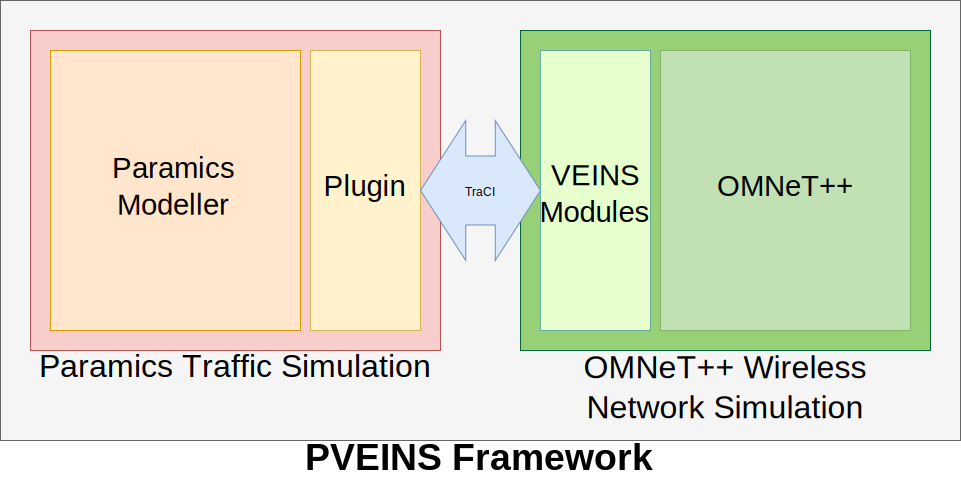
\includegraphics[width=\linewidth]{figuras/PVEINSArch.png}
    \caption{Visión macroscópica del framework; el plugin desarrollado actúa como una interfaz entre TraCI y Paramics.}
    \label{fig:pveins_genarch}
\end{figure}

A nivel más microscópico, la arquitectura del \emph{framework} se desarrolló en dos versiones distintas, la primera de éstas siendo descartada al realizar las pruebas de validación del proyecto. A continuación, se describirán brevemente estas dos iteraciones del diseño del software, destacando principalmente las razones del descarte de la versión preliminar.

\subsubsection{Arquitectura preliminar}

Originalmente, el \emph{framework} se implementó como un hilo de ejecución (un \emph{thread}) paralelo a Paramics. La principal ventaja de este diseño era evitar el bloqueo de la interfaz del simulador al encontrarse el servidor TraCI bloqueado esperando mensajes entrantes en el \emph{socket}. 

Un diagrama de la arquitectura general de esta implementación puede observarse en la figura \ref{fig:ptraci_arch}. Al iniciar Paramics, el \emph{plugin} inicializa el servidor en un \emph{thread} paralelo; el servidor luego se enlaza a un \emph{socket} TCP y se bloquea en espera de mensajes entrantes desde un cliente TraCI (en nuestro caso, VEINS). Al recibir una serie de comandos TraCI, el servidor los interpreta, comunicándose con Paramics a través de su API, obteniendo datos y modificando el estado de la simulación. El servidor interpreta todos los comandos en un mensaje TraCI antes de enviar todos los mensajes de respuesta correspondientes en un único mensaje TraCI.

Esta arquitectura funciona de manera eficiente y permite la ejecución de la simulación de Paramics completamente sin la intervención del usuario (ya que el \emph{thread} mismo del \emph{plugin} era capaz de llamar el método de inicio de simulación). 

Sin embargo, al comenzar a realizar pruebas con redes de tamaño más extenso se presentó un problema imprevisto, y -- a la larga -- irreparable sin acceso al código fuente de Paramics. El problema radica en la función de avance de simulación definido en la API de Paramics, \texttt{qps\_GUI\_runSimulation()}, la cual, como se descubrió, también actualiza la interfaz gráfica de el modelador de Paramics a través de llamados a la librería Qt4 \cite{qt}. Estos llamados no son \emph{thread-safe}\footnote{Es decir, no incluyen medidas para asegurar el acceso exclusivo de recursos a un sólo \emph{thread}.}, y en redes grandes de Paramics generan \emph{data races} al ser invocados desde un \emph{thread} paralelo al principal del simulador. Esto finalmente genera corrupción de memoria en el motor gráfico (principalmente, lecturas de direcciones inválidas de memoria), lo cual causa un error fatal en la simulación.

Se estudiaron múltiples maneras de resolver este problema manteniendo la estructura paralela del \emph{plugin} sin éxito, ya que la única manera confiable de forzar un avance de la simulación desde el \emph{plugin} es a través de la función anteriormente mencionada. Se decidió entonces abordar el problema desde un ángulo distinto, enfoque que se discutirá en la siguiente sección.

\begin{figure}[]
    \centering
    \begin{sequencediagram}
    \newthread{D}{OMNeT++}{}
    \newinst[1]{A}{VEINS}{}
    \newinst[3]{B}{Plugin}{}
    \newthread[3]{C}{Paramics}{}
    
    \begin{messcall}{C}{run()}{B}
        \postlevel
        \begin{call}{B}{waitForCommands()}{B}{}
        \end{call}
    \end{messcall}
    
    \begin{call}{D}{Solicitud}{A}{Resultado}
    
        \begin{call}{A}{Comando TraCI}{B}{Respuesta TraCI}
            \begin{call}{B}{parseCommand()}{B}{sendResponse()}
                \postlevel
                \begin{call}{B}{API Paramics}{C}{Datos}
                \end{call}
                \postlevel
            \end{call}
        \end{call}
    \end{call}
\end{sequencediagram}
    \caption{Arquitectura preliminar}
    \label{fig:ptraci_arch}
\end{figure}

\subsubsection{Arquitectura final} \label{sec:architecture:final}

El problema presentado por la incompatibilidad de \texttt{qps\_GUI\_runSimulation()}, función de avance de simulación de la API de Paramics, con múltiples \emph{threads} implicó la necesidad de reevaluar la arquitectura general del \emph{framework}. Se decidió descartar la idea de un \emph{thread} paralelo para el servidor, y se implementó un esquema secuencial de interpretación de mensajes TraCI, utilizando \emph{loops} bloqueantes para controlar la ejecución de pasos de simulación.

Esta arquitectura puede visualizarse en la figura \ref{fig:ptraci_arch2}. Al principio de cada paso de simulación, el simulador invoca la función \texttt{qpx\_CLK\_startOfSimLoop()}, definida en el \emph{plugin}, antes de realizar cualquier otra acción. Esta función a su vez invoca el método \texttt{preStep()} del servidor, dentro del cual se ejecuta un \emph{loop} de interpretación de comandos TraCI (y de envío de respuestas a éstos). Este \emph{loop} se interrumpe al recibir un mensaje de paso de simulación, retornando así de \texttt{preStep()} y \texttt{qpx\_CLK\_startOfSimLoop()}, y liberando al simulador para que realice su procedimiento interno de avance de simulación. 

Luego de realizar el avance de simulación, Paramics invoca la función \texttt{qpx\_CLK\_endOfSimLoop()}, también definida en el \emph{plugin}. Esta invoca a su vez el método \texttt{postStep()} del servidor, el cual se encarga de realizar la recolección de datos post-paso de simulación, de terminar de interpretar eventuales comandos recibidos previo al paso de simulación y de enviar respuestas pendientes al cliente. Finalmente, esta función retorna el control de la ejecución a Paramics, y el ciclo comienza nuevamente.

Mediante esta arquitectura se logró eliminar por completo el problema presentado por \texttt{qps\_GUI\_runSimulation()}, y ya que todo corre en un sólo \emph{thread}, se evita el uso de elementos de sincronización, los cuales pueden agregar \emph{overhead} al procedimiento.

Este nuevo diseño presenta una única desventaja: es necesario el inicio de la simulación de manera manual por parte del usuario, luego de lo cual funciona de manera autónoma. Esto ya que no existe manera de iniciar el \emph{loop} de simulación de Paramics a través de la API sin recurrir a \emph{threads}.

Finalmente, se debe notar que dada la representación en tiempo discreto de los pasos de simulación, el avance de esta en muchos casos no alcanza exactamente el tiempo deseado. Si definimos el paso de simulación como $\triangle T$, el instante de tiempo en que se recibe el comando de avance como $T_{i}$ y el instante de tiempo objetivo $T_{o}$, la simulación se avanzará un número $n \in \mathbb{N}$ de pasos, tal que

\[ T_{i} + (n \times \triangle T) = T_{f} \]
\[ T_{i} + ((n - 1) \times \triangle T) = T_{f}' \]
\[ T_{f} \geq T_{o} \]
\[ T_{f}' < T_{o} \]

En otras palabras, la simulación se avanzará el mínimo número de pasos tal que el tiempo final es \emph{igual o mayor} al instante de tiempo objetivo. Esto es para asegurar que se ejecuten todas las acciones que dependan del tiempo de simulación por lo menos hasta dicho instante.

\begin{figure}[htpb]
    \centering
    \begin{sequencediagram}
    \newthread{B}{Paramics + Plugin}{}
    \newthread[7]{A}{OMNeT++/VEINS}{}

    \begin{sdblock}{Loop de simulación}{}
        \postlevel
        \begin{call}{B}{\texttt{qpx\_CLK\_startOfSimLoop()}}{B}{}
            \begin{sdblock}{Loop pre-simulación}{}
                \begin{call}{B}{\texttt{server->preStep()}}{B}{Comando: Paso de Simulación}
                    \postlevel
                    \begin{messcall}{A}{Mensajes TraCI}{B}
                    \end{messcall}
                    \begin{messcall}{B}{Respuestas TraCI}{A}
                    \end{messcall}
                \end{call}
            \end{sdblock}
        \end{call}
        \begin{sdblock}{Paso de simulación}{}
            \postlevel
            \postlevel
            \begin{call}{B}{\begin{minipage}{8cm}
                        Actualización de estado:
                        \begin{itemize}
                            \item Salida y llegada de vehículos
                            \item Modificación de velocidades y rutas
                        \end{itemize}
                \end{minipage}}{B}{}
            \end{call}
        \end{sdblock}
        \postlevel
        \begin{call}{B}{\texttt{qpx\_CLK\_endOfSimLoop()}}{B}{}
            \begin{sdblock}{Loop post-simulación}{}
                \begin{call}{B}{\texttt{server->postStep()}}{B}{Fin de Comandos}
                    \postlevel
                    \begin{messcall}{B}{Respuestas TraCI}{A}
                    \end{messcall}
                \end{call}
            \end{sdblock}
        \end{call}
    \end{sdblock}
\end{sequencediagram}
    \caption{Arquitectura final del \emph{framework}}
    \label{fig:ptraci_arch2}
\end{figure}
\newpage
\section{Metodología de desarrollo} \label{sec:metodologia}

El desarrollo del \emph{plugin} se llevó a cabo de manera iterativa, implementando funcionalidades esenciales en primera instancia, y luego construyendo sobre esta base, cuidando en cada paso de no pasar a llevar las funcionalidades previamente implementadas y perfeccionando implementaciones anteriores. El orden de desarrollo de las funcionalidades fue cuidadosamente planeado, tomando en cuenta que en muchos casos se requería un orden específico de implementación de funcionalidades; \emph{e.g.} era imperativo el desarrollo de la funcionalidad de obtención de variables de vehículos antes de poder implementar suscripciones, ya estas últimas dependen de la funcionalidad de la primera. Las etapas generales de desarrollo que se siguieron fueron:

\begin{enumerate}
    \item En primer lugar, se desarrolló la base de comunicaciones del \emph{framework}, es decir, comunicación con el \emph{socket}, recepción e interpretación de mensajes. 
    
    \item A continuación, se implementó la funcionalidad esencial de control de simulación (los comandos presentados en la sección \ref{sec:comandos:controlsim}), con el fin de poder establecer una primera conexión con un cliente TraCI y simplemente ejecutar una simulación sin otros comandos. 
    El protocolo define un ``\emph{handshake}'' consistente en la verificación de versiones de TraCI compatibles entre cliente y servidor, por lo que el correcto funcionamiento del comando de obtención de versión fue prioridad en esta etapa.
    
    \item Se implementaron los comandos de obtención de variables de la simulación. Teniendo ya la base de comunicaciones funcionando, la implementación de éstos fue mucho más directa.
    
    \item Sobre la implementación de los comandos de obtención de variables, se desarrollaron los distintos tipos de suscripciones disponibles.
    
    \item Finalmente, en última instancia, se desarrollaron los comandos de modificación de estados, ya que éstos necesariamente requerían una fundación sólida dada su relativa complejidad.
\end{enumerate}

Cabe destacar que, pese a la cuidadosa planificación realizada previa al desarrollo del \emph{framework} (y como siempre sucede en el desarrollo de \emph{software}), en muchas oportunidades fue necesario volver a un paso anterior para rediseñar o mejorar una implementación. El principal ejemplo de ésto es el rediseño de la arquitectura general del \emph{plugin}, detallado en la sección \ref{sec:architecture}, el cual implicó el rediseño y posterior reimplementación de gran parte de las etapas 1 (base de comunicaciones) y 2 (funcionalidad de control de simulación) del \emph{plugin}.

En términos de control de versiones y manejo del historial del desarrollo se escogió utilizar el sistema \emph{git} \autocite{git}, dada su popularidad, extenso soporte y documentación y la familiaridad del memorista con este sistema. El servicio de \emph{hosting} específico escogido para el sistema fue \emph{GitHub} \autocite{github}; el código fuente del proyecto puede encontrarse en el perfil personal del autor \autocite{molguin_github}, en el repositorio \autocite{pveins_github}.
\newpage
\section{Funcionalidad implementada}\label{sec:functionality}

El protocolo TraCI define más de 30 comandos distintos, cada uno con una gran cantidad de variables y parámetros asociados (ver apéndice \ref{anex:traci} para una descripción más detallada del funcionamiento de este protocolo). La implementación de todas las funcionalidades está fuera del alcance de esta memoria, por lo que se escogió un subconjunto acotado de éstas a implementar, considerando en específico aquellos comandos esenciales para simulaciones de ITS que contribuyen al cumplimiento del objetivo general de esta memoria.

\subsection{Comandos Implementados} \label{sec:comandos}

\subsubsection{Comandos de Control de Simulación}\label{sec:comandos:controlsim}

\begin{itemize}
    \begin{multicols}{2}
        \mcitem{\texttt{0x00} Obtención de Versión}
        \mcitem{\texttt{0x02} Avance de Simulación}
        \mcitem{\texttt{0xff} Cierre de Conexión}
    \end{multicols}
\end{itemize}

\subsubsection{Comandos de Obtención de Variables}

\begin{description}[style=multiline]
    
    \item[\texttt{0xa4}] Variables de vehículos
    \begin{multicols}{2}
        \begin{itemize}
            \mcitem{\texttt{0x00} Lista de vehículos activos en la red}
            \mcitem{\texttt{0x01} Número de vehículos activos en la red}
            \mcitem{\texttt{0x36} Inclinación actual}
            \mcitem{\texttt{0x39} Posición actual (3D)}
            \mcitem{\texttt{0x40} Velocidad actual}
            \mcitem{\texttt{0x42} Posición actual (2D)}
            \mcitem{\texttt{0x43} Ángulo actual}
            \mcitem{\texttt{0x44} Largo}
            \mcitem{\texttt{0x4d} Ancho}
            \mcitem{\texttt{0x4f} Tipo de vehículo}
            \mcitem{\texttt{0x50} Calle actual}
            \mcitem{\texttt{0x51} Identificador de pista actual}
            \mcitem{\texttt{0x52} Índice de pista actual}
            \mcitem{\texttt{0xbc} Altura}
        \end{itemize}
    \end{multicols}
    
    \item[\texttt{0xa5}] Variables de tipos de vehículos
    \begin{multicols}{2}
        \begin{itemize}
            \mcitem{\texttt{0x00} Lista de tipos definidos}
            \mcitem{\texttt{0x01} Número de tipos definidos}
            \mcitem{\texttt{0x41} Velocidad máxima}
            \mcitem{\texttt{0x44} Largo}
            \mcitem{\texttt{0x46} Aceleración máxima}
            \mcitem{\texttt{0x47} Deceleración máxima}
            \mcitem{\texttt{0x4d} Ancho}
            \mcitem{\texttt{0xbc} Altura}
        \end{itemize}
    \end{multicols}
    
    \item[\texttt{0xa6}] Variables de rutas
    \begin{multicols}{2}
        \begin{itemize}
            \mcitem{\texttt{0x00} Lista de rutas definidas}
            \mcitem{\texttt{0x01} Número de rutas definidas}
            \mcitem{\texttt{0x54} Arcos (calles) componentes de la ruta}
        \end{itemize}
    \end{multicols}
    
    \item[\texttt{0xa8}] Variables de polígonos (edificios y estructuras)
    \begin{multicols}{2}
        \begin{itemize}
            \mcitem{\texttt{0x00} Lista de polígonos}
            \mcitem{\texttt{0x01} Número de polígonos}
        \end{itemize}
    \end{multicols}
    
    Cabe notar que Paramics no maneja edificios en sus simulaciones, al menos no edificios accesibles a través de la API de programación, por lo que estos métodos se implementaron de manera que reportan siempre 0 polígonos en la simulación.
    
    \item[\texttt{0xa9}] Variables de nodos (intersecciones) de la red
    \begin{multicols}{2}
        \begin{itemize}
            \mcitem{\texttt{0x00} Lista de intersecciones}
            \mcitem{\texttt{0x01} Número de intersecciones}
            \mcitem{\texttt{0x42} Posición de la intersección}
        \end{itemize}
    \end{multicols}
    
    \item[\texttt{0xaa}] Variables de arcos (calles) de la red
    \begin{multicols}{2}
        \begin{itemize}
            \mcitem{\texttt{0x00} Lista de calles}
            \mcitem{\texttt{0x01} Número de calles}
        \end{itemize}
    \end{multicols}
    
    \item[\namedlabel{item:simvars}{\texttt{0xab}}] Variables de Simulación
    \begin{multicols}{2}
        \begin{itemize}
            \mcitem{\texttt{0x70} Tiempo de simulación}
            \mcitem{\texttt{0x73} Número de vehículos liberados a la red en el último paso de simulación}
            \mcitem{\texttt{0x74} Lista de vehículos liberados a la red en el último paso de simulación}
            \mcitem{\texttt{0x79} Número de vehículos que han llegado a su destino en el último paso de simulación}
            \mcitem{\texttt{0x7a} Lista de vehículos que han llegado a su destino en el último paso de simulación}
            \mcitem{\texttt{0x7b} Tamaño del paso de simulación}
            \mcitem{\texttt{0x7c} Coordenadas de los límites de la red vehicular}
        \end{itemize}
    \end{multicols}
    
    Las variables \texttt{0x75}, \texttt{0x76}, \texttt{0x77} y \texttt{0x78}, correspondientes a los números y listas de vehículos que comienzaron y terminaron de teletransportarse en el último paso de simulación, así como las variables \texttt{0x6c}, \texttt{0x6d}, \texttt{0x6e} y \texttt{0x6f}, las cuales corresponden a números y listas de vehículos que comenzaron y terminaron de estar estacionados, fueron implementadas ``parcialmente''. En estricto rigor, los mecanismos subyacentes no se implementaron porque no se consideraron críticos, pero se implementó una respuesta \emph{dummy} de 0 vehículos para asegurar su funcionamiento con VEINS.
    
\end{description}

\subsubsection{Comandos de modificación de estado}\label{sec:mod_state}

\begin{description}[style=multiline]
    \item [\texttt{0xc4}] Variables de vehículo
    \begin{multicols}{2}
        \begin{itemize}
            \mcitem{\texttt{0x13} Cambio de pista}
            \mcitem{\texttt{0x14} Cambio de velocidad (lineal)}
            \mcitem{\texttt{0x40} Cambio de velocidad (instantáneo)}
            \mcitem{\texttt{0x41} Cambio de velocidad máxima}
            \mcitem{\texttt{0x45} Coloreado}
            \mcitem{\texttt{0x57} Cambio de ruta (a una lista de arcos otorgada por el cliente)}
            
        \end{itemize}
    \end{multicols}
\end{description}
%\chapter{Implementación}\label{cap:implementation}


\chapter{Validación}\label{cap:validacion}

La implementación del \emph{plugin} se sometió a un conjunto de diversas pruebas para verificar su correcto funcionamiento y la eficiencia del \emph{framework}. Estas pruebas consistieron en la simulación de escenarios realistas, de idéntica complejidad a aquellos escenarios para los que fue concebido y diseñado. 

\minitoc

\section{Escenario y Análisis}\label{sec:experiments}
\subsection{Escenario modelado}

\begin{figure}[tpb]
    \centering
    \begin{subfigure}{0.8\textwidth}
        \centering
        \includegraphics[width=\linewidth]{figuras/costanera.png}
        \caption{Mapa en Paramics del escenario simulado.}
    \end{subfigure}\\
    \begin{subfigure}{0.8\textwidth}
        \centering
        \includegraphics[width=\linewidth]{figuras/costanera_maps.png}
        \caption{Escenario simulado en la ``vida real'', Google Maps.}
    \end{subfigure}
    \caption{Escenario modelado, Paramics vs. ``vida real''.}
    \label{fig:costanera}
\end{figure}

Como escenario de transporte para la validación del \emph{framework} se utilizó un modelo de un sector de la ciudad de Santiago de Chile, el cual consiste en una simulación detallada del flujo vehicular en la comuna de Providencia. Este modelo fue creado en 2010 por Víctor Zúñiga para el desarrollo de su memoria de grado \autocite{zuniga}, y simula el impacto sobre el sector entre las avenidas Providencia, Tobalaba, Andrés Bello y Santa María proyectado en ese entonces por la construcción de un nuevo centro comercial (ver figura \ref{fig:costanera}).

Sobre este escenario vehicular se construyó un modelo de ITS, utilizando el \emph{plugin} desarrollado y el \emph{framework} VEINS en OMNeT++. Este consistió en un escenario en que un vehículo sufre un desperfecto en una cierta calle de la simulación y emite \emph{beacons} de advertencia en \emph{broadcast} a todos los demás vehículos que se encuentran dentro del alcance de la transmisión. A aquellos vehículos que reciben un \emph{beacon}, y que se puede predecir ingresarán a a la calle en que se encuentra el vehículo averiado, se les modifica luego su ruta mediante VEINS y TraCI.

De manera más detallada, el escenario funciona de la siguiente manera:

\begin{enumerate}
    \item Al iniciarse el \emph{framework}, OMNeT++ (utilizando VEINS) inicializa una conexión TraCI con el \emph{plugin} en Paramics.
    \item Por cada vehículo que ingresa a la red de transporte, OMNeT++ crea un módulo dotado de lógica y capacidades comunicaciones en su simulación de red, y asocia el movimiento de este módulo al vehículo en Paramics. En adelante, se entenderá por ``vehículo'' el par consistente en el vehículo en Paramics y su módulo asociado en OMNeT++.
    \item Periódicamente se verifica la posición de cada vehículo, y al detectar el primero en ingresar a la calle del ``accidente'', este es detenido. La calle en cuestión para esta simulación fue el arco ``40:5'', el cual corresponde a Avenida Vitacura, frente al centro comercial. El vehículo además se colorea rojo para su fácil identificación.
    \item El módulo OMNeT++ del vehículo accidentado emite luego, cada 5 segundos, un mensaje WAVE \autocite{80211wave} en \emph{broadcast}.
    \item Aquellos vehículos que reciban el \emph{beacon} de emergencia, se encuentren en alguna de las calles aledañas al accidente y que tengan un destino que probablemente los haga pasar por la calle afectada, cambian su ruta a utilizar el arco ``40:7'', correspondiente a la calle Holanda, entre Avda. Vitacura y Avda. Providencia. Además, se cambia su color a púrpura para visualizarlos de manera más fácil en Paramics.
\end{enumerate}

Esta simulación dura un total de \textbf{15 minutos de tiempo \emph{simulado}}, y se ejecutó con múltiples configuraciones del sistema de transporte y del sistema de comunicaciones, las cuales se verán a continuación en las secciones \ref{sec:results:performance} y \ref{sec:results:vehicular}. Las especificaciones técnicas del equipo en donde se realizaron estos experimentos pueden observarse en la tabla \ref{table:systemspecs}.

\begin{table}[tpb]
    \centering
    \begin{tabular}{@{}ll@{}}
        \toprule
        Sistema Operativo     & Windows 10 v.10.0.14393         \\
        Procesador            & Intel Core i7 4720HQ @ 2.60 GHz \\
        N$^{o}$ de Núcleos / Threads & 4 núcleos / 8 threads\\
        Arquitectura          & x86\_64                         \\
        RAM                   & 12 GB DDR3L 1600 MHz            \\
        Tarjeta de Video      & NVIDIA GeForce GTX 960M         \\
        Memoria Video         & 2 GB GDDR5                      \\ \bottomrule
    \end{tabular}
    \caption{Especificaciones técnicas del entorno de simulación.}
    \label{table:systemspecs}
\end{table}

Las mediciones realizadas se enfocaron a probar el funcionamiento del \emph{framework} en dos categorías de análisis; \textbf{eficiencia computacional} de la implementación e \textbf{impacto sobre el modelo de transporte}. De esta manera se pretende demostrar que PVEINS es una opción viable para la investigación en Sistemas Inteligentes de Transporte, tanto en términos de los recursos que utiliza el \emph{framework} para la ejecución de las simulaciones como en términos de la validez de los resultados obtenidos.

Los resultados obtenidos de cada simulación fuero exportados desde OMNeT++ a archivos CSV, los cuales luego se analizaron utilizando Python 3.6.
Se utilizaron las librerías Pandas \autocite{pandas}, para el manejo de los datos de manera eficiente, Numpy \autocite{numpy}, para cálculos, y Matplotlib \autocite{matplotlib} y matplotlib2tikz \autocite{matplotlib2tikz} para la generación de gráficos que permitiesen analizar los datos de manera más efectiva e intuitiva.


\section{Eficiencia Computacional}\label{sec:results:performance}
\subsection{Mediciones Realizadas}

El principal factor a medir en esta categoría es la relación entre la cantidad de vehículos en una simulación y el tiempo real que demora el \emph{framework} en simular el escenario, para una duración en tiempo simulado específica. De esta manera, se pretende caracterizar el comportamiento del \emph{software} para escenarios vehiculares de alta complejidad, en los cuales pueden llegar a interactuar miles de vehículos. Además, interesa también la carga en términos de recursos de sistema que genera la ejecución de la simulación sobre el equipo de prueba. 

A través de éstos datos se pretende generar un perfil del \emph{software} que indique los requisitos que impone sobre el entorno de simulación, y su factibilidad de uso para sistemas de transporte complejos tanto en entornos de simulación de alto rendimiento como de mediano y bajo.

Antes de detallar las simulaciones realizadas, se debe definir el término \emph{factor de demanda}. Éste corresponde a un elemento de configuración de la simulación de transporte en Paramics, el cual caracteriza la carga vehicular sobre el sistema de transporte en cada instante de tiempo. En términos más simples, el factor de demanda regula la cantidad de vehículos que Paramics inserta a la red durante la simulación; es un valor porcentual cuya correspondencia en cantidad real de vehículos en la red dependerá de las características particulares de cada simulación. Sin embargo, los valores aproximados para el escenario utilizado, para distintos factores de demanda, pueden observarse en la tabla \ref{table:demandfactor}.

Se realizaron entonces 16 ejecuciones del escenario (de aquí en adelante, denominadas \emph{runs}) con cuatro factores de demanda distintos (4 \emph{runs} con 100\%, 4 con 75\%, 4 con 50\% y 4 con 25\%) y cada una con una \emph{semilla} distinta para los generadores de números pseudoaleatorios. De éstos \emph{runs} se extrajeron las siguientes estadísticas:

\begin{enumerate}
    \item Timestamp de inicio del \emph{run}.
    \item Timestamp de fin del \emph{run}.
    \item Duración en tiempo real del \emph{run}.
    \item Cantidad de vehículos en la red de transporte, cada 1 minuto de tiempo simulado.
\end{enumerate}

Además, se realizó una ejecución adicional de un \emph{run} con factor de demanda 100\%, y se midió la carga sobre el equipo de prueba mientras se ejecutaba la simulación utilizando las herramientas de monitoreo de sistema de Microsoft Windows. En específico, se midió la carga porcentual sobre el procesador, la memoria RAM utilizada y la cantidad de operaciones de escritura y lectura del disco físico durante la simulación.

\begin{table}[htpb]
    \centering
    \begin{tabular}{@{}rrr@{}}
        \textbf{Factor de Demanda} & \textbf{Ctdad. Prom. Vehículos} \\ \midrule
        100\%           & 1379.9 \\ %\midrule
        75\%            & 868.75 \\ %\midrule
        50\%            & 514.5825 \\ %\midrule
        25\%            & 246.5675 \\ \bottomrule
    \end{tabular}
    \caption[Factor de demanda vs. cantidad promedio de vehículos]{Tabla de relación entre factor de demanda y cantidad promedio de vehículos por instante de tiempo en el escenario de prueba.}
    \label{table:demandfactor}
\end{table}

\subsection{Resultados}

\subsubsection{Duración de la Simulación}

La tabla \ref{table:vehiclesvstime} presenta los resultados obtenidos del tiempo de duración de la simulación versus la cantidad de vehículos promedio por instante de tiempo; estos datos se visualizan además de manera gráfica en la figura \ref{fig:vehiclesvstime}.

\begin{table}[htpb]
    \centering
    \begin{tabular}{@{}rrr@{}}
        \textbf{Factor de Demanda} & \textbf{Nro. Prom. Vehículos} & \textbf{Tiempo Promedio [s]} \\ \midrule
        100\%           & 1379.9          & 1471.5              \\ %\midrule
        75\%            & 868.75          & 683.5               \\ %\midrule
        50\%            & 514.5825        & 275.75              \\ %\midrule
        25\%            & 246.5675        & 113.25              \\ \bottomrule
    \end{tabular}
    \caption[Cantidad de vehículos vs. tiempo real de simulación]{Promedio cantidad de vehículos en simulación (por instante de tiempo) vs. tiempo promedio de simulación, 15 minutos de tiempo simulado.}
    \label{table:vehiclesvstime}
\end{table}

\begin{figure}[htpb]
    \centering    
    \input{figuras/n_vhcs_vs_time.tex}
    \captionof{figure}[Cantidad de vehículos vs. tiempo real de simulación]{Gráfico de dispersión del promedio de vehículos en simulación por instante de tiempo vs. tiempo total de simulación, para una simulación de 15 minutos de tiempo simulado.}
    \label{fig:vehiclesvstime}
\end{figure}

De estos resultados se puede concluir que el \emph{framework}, como era de esperarse dada la naturaleza de la simulación, presenta una relación levemente exponencial entre la cantidad promedio de nodos en la red vehicular con el tiempo que efectivamente demora una simulación en completar su ejecución.

Se utilizó numpy para calcular un ajuste polinomial a los datos obtenidos, obteniendo la siguiente relación entre cantidad de vehículos promedio en la simulación $N_{v}$ y tiempo de ejecución de ésta en segundos, $T(N_{v})$:

\[ T(N_{v}) = (5.829 \times 10^{-4})N_{v}^{2} + (2.586 \times 10^{-1})N_{v} + 6.317 \]

Esto indica que a pesar de ser exponencial, la relación presenta una curva bastante suavizada. Es factible entonces simular escenarios de escala aún mayor que la presentada en esta memoria (la cual, cabe notar, no es menor), sin mayores dificultades.

La figura \ref{fig:timevsvehicles_evolution} presenta por lo otro lado la evolución de la red vehicular en términos de cantidad de vehículos para un \emph{run} con factor de demanda de 100\%, tanto en tiempo real como en tiempo simulado. Este gráfico permite visualizar además como la cantidad de vehículos en la red afecta el tiempo de ejecución de cada paso de simulación.

\begin{figure}[htpb]
    \centering
    \input{figuras/timevsvehicles_evolution.tex}
    \caption[Evolución temporal de la cantidad de vehículos en la simulación.]{Evolución de la cantidad de vehículos en una simulación con factor de demanda 100\%, para tiempo real y simulado.}
    \label{fig:timevsvehicles_evolution}
\end{figure}

\subsubsection{Carga computacional}

En términos de carga sobre el entorno de simulación, se pueden observar los resultados obtenidos en las figuras \ref{fig:systemload:cpuram} y \ref{fig:systemload:io}. 

\begin{figure}[htpb]
    \centering
    \input{figuras/system_performance.tex}
    \caption{Carga sobre el sistema durante una simulación con factor de demanda 100\%.}
    \label{fig:systemload:cpuram}
\end{figure}

La figura \ref{fig:systemload:cpuram} ilustra la carga sobre el sistema en términos porcentuales. En específico, se puede observar como el uso promedio del procesador aumenta en aproximadamente un 20\% durante la simulación, situación fácilmente manejable para cualquier procesador moderno. Además, el uso de memoria aumenta en menos de un 5\% -- en términos numéricos, el sistema utiliza menos de 600 MB para simular un escenario con un promedio de 1400 nodos presentes en cualquier instante, lo cual es un valor muy razonable si se considera que el estándar de memoria RAM para computadores personales hoy en día es por lo menos 4 GB \autocite{steamhwsurvey, unityhardwaresurvey}.

Por otro lado, la figura \ref{fig:systemload:io} ilustra el uso del disco duro del sistema durante la ejecución de la simulación. 
Cabe destacar que durante el \emph{run} en cuestión se extrajeron y almacenaron un gran número de estadísticas en cada instante de simulación, las cuales OMNeT++ almacena directamente en el disco. 
Sin embargo, aún así, se puede notar que el \emph{framework} es austero en su utilización de los recursos del sistema.

\begin{figure}[htpb]
    \centering
    \input{figuras/system_io.tex}
    \caption[I/O en disco durante simulación]{Lecturas y escrituras de disco por segundo durante una simulación con factor de demanda 100\%.}
    \label{fig:systemload:io}
\end{figure} 
\section{Modelo Vehicular}

\begin{figure}
    \centering
    % This file was created by matplotlib2tikz v0.6.10.
\begin{tikzpicture}

\begin{axis}[
xlabel={Factor de Demanda},
xmin=-0.22, xmax=2.42,
ymin=0, ymax=5000,
width=\figurewidth,
height=\figureheight,
xtick={0.1,1.1,2.1},
xticklabels={20\%,50\%,100\%},
tick align=outside,
tick pos=left,
xmajorgrids,
x grid style={lightgray, opacity=0.7},
ymajorgrids,
y grid style={lightgray, opacity=0.7},
axis line style={black, opacity=0.0},
legend cell align={left},
legend style={at={(0.03,0.97)}, anchor=north west, draw=white!80.0!black, fill=white!89.803921568627459!black},
legend entries={{Sin comunicaci\'on},{Con comunicaci\'on}}
]
\addlegendimage{ybar,ybar legend,fill=red,draw opacity=0};
\draw[fill=red,draw opacity=0] (axis cs:-0.1,0) rectangle (axis cs:0.1,985);
\draw[fill=red,draw opacity=0] (axis cs:0.9,0) rectangle (axis cs:1.1,2441);
\draw[fill=red,draw opacity=0] (axis cs:1.9,0) rectangle (axis cs:2.1,3801);
\addlegendimage{ybar,ybar legend,fill=blue,draw opacity=0};
\draw[fill=blue,draw opacity=0] (axis cs:0.1,0) rectangle (axis cs:0.3,1009);
\draw[fill=blue,draw opacity=0] (axis cs:1.1,0) rectangle (axis cs:1.3,2512);
\draw[fill=blue,draw opacity=0] (axis cs:2.1,0) rectangle (axis cs:2.3,3858);
\node at (axis cs:-0.05,1025)[
scale=1.0,
anchor=west,
text=black,
rotate=45.0
]{ 985};
\node at (axis cs:0.95,2481)[
scale=1.0,
anchor=west,
text=black,
rotate=45.0
]{ 2441};
\node at (axis cs:1.95,3841)[
scale=1.0,
anchor=west,
text=black,
rotate=45.0
]{ 3801};
\node at (axis cs:0.15,1049)[
scale=1.0,
anchor=west,
text=black,
rotate=45.0
]{ 1009};
\node at (axis cs:1.15,2552)[
scale=1.0,
anchor=west,
text=black,
rotate=45.0
]{ 2512};
\node at (axis cs:2.15,3898)[
scale=1.0,
anchor=west,
text=black,
rotate=45.0
]{ 3858};
\end{axis}

\end{tikzpicture}
    \caption[Cantidad de vehículos que alcanzaron su destino]{Comparación cantidad de vehículos que alcanzaron su destino en 15 minutos de tiempo simulado con tres factores de demanda distintos.}
    \label{fig:arrivedcomp}
\end{figure}

\begin{figure}[htpb]
    \centering
    \input{figuras/per00per10_timedistance.tex}
    \caption{Gráfico de dispersión, distancia total vs tiempo, para escenarios con PER 0.0 y PER 1.0}
    \label{fig:distvstime}
\end{figure}

\begin{figure}[htpb]
    \centering
    \input{figuras/per00per10_co2.tex}
    \caption{Gráfico de dispersión, distancia total vs CO$^{2}$ total, para escenarios con PER 0.0 y PER 1.0}
    \label{fig:distvsco2}
\end{figure}

\begin{table}[htpb]
    \centering
    \begin{tabular}{@{}l|rrr@{}}
        \multicolumn{1}{c|}{\textbf{Duración}} & \multicolumn{1}{c}{\begin{tabular}[c]{@{}c@{}}\textbf{Alcanzaron destino}\\ \textbf{PER 0.0}\end{tabular}} & \multicolumn{1}{c}{\begin{tabular}[c]{@{}c@{}}\textbf{Alcanzaron destino}\\ \textbf{PER 1.0}\end{tabular}} & \multicolumn{1}{c}{$\triangle$} \\ \midrule
        15 min & 3858 & 3801 & 57 \\
        120 min & 11488 & 11014 & 474 \\ \bottomrule
    \end{tabular}
    \caption{My caption}
    \label{my-label}
\end{table}
\chapter{Conclusiones}
\section{Cumplimiento de objetivos}\label{sec:conclusiones:obj}

El objetivo general del presente trabajo de memoria, ``\textbf{el desarrollo de un \textit{framework} de integración entre un simulador de redes, OMNeT++ y un microsimulador de tráfico, Quadstone Paramics, de tal manera que exista comunicación bidireccional entre ambos}'', fue logrado en su totalidad. PVEINS, el \emph{framework} desarrollado, permite la integración totalmente transparente de Paramics con el \emph{framework} VEINS, desarrollado por Sommer \emph{et al.} en \autocite{sommer_german_dressler}, y OMNeT++, posibilitando así la simulación de Sistemas de Transporte Inteligentes complejos, además del uso de la gran cantidad de modelos de comunicación ya desarrollados para dicho simulador de redes de comunicaciones. 
Se logró esta integración mediante la implementación de un \emph{plugin} para Paramics, el cual actúa como una interfaz entre el simulador y el protocolo TraCI, permitiendo así el intercambio estandarizado de información y comandos con OMNeT++ y VEINS a través de un \emph{socket} TCP. 

Se demostró además que esta implementación es altamente eficiente en términos de la relación entre tiempo de duración real y tiempo simulado para simulaciones de gran tamaño, del orden de cientos o hasta miles de nodos presentes simultáneamente en la red. 
La implementación es también austera en recursos de sistema, utilizando menos de 600 MB de memoria y aumentando la actividad del procesador en un 20\% para una simulación con un promedio de 1400 nodos activos en cualquier instante dado.

En términos de los objetivos particulares enumerados en la sección \ref{sec:obj:part}, se puede concluir que:

\begin{enumerate}
    \item \textbf{Se estableció el estado del arte en cuanto a simulación bidireccional en comunicaciones inalámbricas y sistemas de transporte}, tomando en cuenta herramientas tanto de código abierto como cerrado. Esto se expuso de manera extensa y profunda en la sección \ref{sec:state_of_the_art}.
    
    \item \textbf{Se escogió la opción de adaptar el \emph{framework} VEINS como solución al problema presentado}, dado que correspondía a la opción más madura y flexible en términos de simulación bidireccional. El razonamiento completo detrás de esta decisión se encuentra en la sección \ref{sec:solution}.
    
    \item \textbf{Se adaptó Paramics}, mediante la implementación de un \emph{plugin}, \textbf{para que pudiese comunicarse de manera bidireccional con OMNeT++}. Se implementaron además todas las funcionalidades enumeradas en la sección \ref{sec:functionality}, las cuales incluyen:
    \begin{enumerate}
        
        \item Construcción de la topología del modelo de comunicaciones a partir de la topología del modelo de tráfico.
        
        \item Actualización dinámica de los nodos en OMNeT++, siguiendo los movimientos de los elementos de Paramics.
        \item Modificación del comportamiento de los nodos del modelo de transporte a partir de eventos en OMNeT++.
    \end{enumerate}
    \item \textbf{Se implementó el \emph{framework} PVEINS siguiendo patrones y buenas prácticas de ingeniería de software} -- el detalle de esto se encuentra en el capítulo \ref{cap:diseno}.
    
    \item \textbf{Se probó y validó el funcionamiento de la integración de los simuladores} mediante la simulación de un modelo de transporte simple pero dinámico (ver sección \ref{sec:simpletest}).
    
    \item Finalmente, \textbf{se implementó un modelo avanzado de transporte}, y se utilizó para \textbf{la evaluación del rendimiento del software implementado y su aplicabilidad a modelos realistas de Sistemas de Transporte Inteligentes}. El detalle del modelo desarrollado y los resultados obtenidos se expusieron en el capítulo \ref{cap:validacion}.
\end{enumerate}
\newpage
\section{Trabajo futuro}

El \emph{framework} desarrollado cumple con todos los objetivos que se expusieron al principio del presente documento, y se evalúa como altamente aplicable para el estudio de modelos de Sistemas Inteligentes de Transporte; sin embargo, aún así queda trabajo futuro por desarrollar. 

Lo más evidente, en primer lugar, es la implementación de los comandos TraCI restantes, los cuales no fueron considerados dentro del alcance de la presente memoria. Estos comandos incluyen diversas acciones no esencialmente necesarias para la simulación de ITS, pero que en un futuro pudiesen llegar a ser requeridos. Comandos como para, por ejemplo, modificar el comportamiento de peatones, semáforos y hasta detectores de bucle de inducción, se encuentran definidos en el protocolo y, de llegar a necesitarse, deberán ser implementados en el \emph{framework}. 
Se debe también tener en consideración la constante evolución de TraCI -- el protocolo se actualiza periódicamente en conjunto con VEINS, y cada nueva versión puede introducir comandos nuevos o deprecar o modificar totalmente comandos antiguos (reemplazándolos con nuevas versiones). Será necesario entonces mantener actualizado PVEINS con estos cambios constantes si se desea mantener compatibilidad con VEINS en el futuro. 
De esta misma manera, se deberá actualizar el \emph{plugin} de Paramics en el caso de actualizaciones que rompan compatibilidad con el API de extensión actual.

En segundo lugar, se plantea la necesidad a futuro de implementar el inicio automático de la simulación de Paramics al recibir una conexión entrante por el \emph{socket} TCP. Esta funcionalidad estaba presente en la primera versión de la arquitectura del \emph{software}, sin embargo fue necesario descartarla al realizar las modificaciones necesarias para el correcto funcionamiento \emph{single-thread} del \emph{plugin} (ver sección \ref{sec:architecture}). Contar con esta funcionalidad significaría poder ejecutar \emph{batches} (conjuntos) de \emph{runs} de simulaciones sin ninguna intervención del usuario -- permitiendo así realizar análisis mucho más acabados de manera más simple.

El \emph{plugin} todavía admite optimización, a pesar de que se trató de implementar de la manera más óptima posible y se realizaron revisiones y reimplementaciones de funcionalidades al descubrir nuevas maneras de optimizar el funcionamiento de éstas. Por ejemplo, la funcionalidad de cambio de pista utiliza una colección aparte para almacenar los comandos de cambios recibidos, sobra la cual se itera luego de cada paso de simulación. 
Esto significa que Paramics, aparte de actualizar el estado de los $N$ vehículos presentes en la simulación en cualquier instante de acuerdo a su modelo interno, deberá recorrer un máximo de otros $N$ elementos adicionales (máximo un cambio de pista por vehículo) y ejecutar los cambios correspondientes después de cada paso de simulación.
De lograrse implementar entonces una versión del cambio de pista similar a las implementaciones de cambio de ruta y velocidad que se llevaron a cabo en el \emph{framework}, es decir, utilizando el mismo modelo de Paramics para realizar los cambios, podría mejorarse el rendimiento, tal vez de manera considerable para escenarios con una gran cantidad de cambios de pista. 

También existen leves ineficiencias en los procesos de recepción e interpretación de mensajes TraCI, las cuales fueron introducidas intencionalmente para aumentar la modularidad y extensibilidad del código. 
Decisiones de diseño como la encapsulación de cada comando en un objeto \texttt{tcpip::Storage} aparte agregan \emph{overhead} al \emph{software} a cambio de código más legible y flexible, factores que en el futuro pueden ser menos importantes que el rendimiento del \emph{framework}. En ese caso, será necesaria una completa refactorización de la estructura interna de paso de parámetros del código, ya esto fue una decisión de diseño fundamental en la implementación actual.

Finalmente, el \emph{framework} podría ser evaluado y analizado por alguien con más experiencia en el área de transporte. En específico, sería valioso un estudio de la validez de los resultados de PVEINS con un escenario que implemente un modelo de re-enrutamiento más avanzado y realista que el empleado para el escenario de validación del presente trabajo de memoria.

%\nocite{*} %incluye todas las citas en la bibliografia, aunque no se hayan referenciado
\blankpage
%\cleardoublepage
%\begin{multicols*}{2}
    %\bibliographystyle{ieeetr}
    %\bibliography{bibliografia}
    %\printbibliography
%\end{multicols*}

\printbibliography[heading=bibintoc]
%\begin{multicols*}{1}[]%\printbibheading]
    
%\end{multicols*}
\blankpage
\appendix
\input{capitulos/anexos/traci.tex}
\chapter{Paramics API} \label{anex:paramics_api}

La API de Paramics consiste en un conjunto de \emph{headers} de código \texttt{C}, los cuales definen un conjunto de funciones accesibles (o incluso, que pueden ser sobrescritas) por \emph{plugins} para el simulador. A continuación se describirán de manera resumida las distintas categorías de funciones expuestas por el \emph{software}.

En primer lugar, los nombres de los métodos de la API siguen el siguiente patrón:
\begin{center}
    \texttt{CATEGORIA\_DOMINIO\_nombre\_de\_funcion()}
\end{center}

\texttt{CATEGORIA} y \texttt{DOMINIO} corresponden a identificadores de tres caracteres, los cuales indican el tipo de función (por ejemplo, de obtención de valores) y su dominio (\emph{e.g.} vehículos o calles).

\section{Categorías de Funciones}

Se definen cuatro categorías de funciones:

\begin{itemize}
    \item Funciones de \emph{override}, prefijo \texttt{QPO}
    \item Funciones de extensión, prefijo \texttt{QPX}
    \item Funciones de obtención de valores, prefijo \texttt{QPG}
    \item Funciones de modificación de valores, prefijo \texttt{QPS}
\end{itemize}

\subsection{Funciones \texttt{QPO}}

Las funciones de \emph{override}, con prefijo \texttt{QPO}, corresponden a funciones que controlan algún comportamiento clave del modelo interno de Paramics y que son sobrescribibles por el usuario. Por ejemplo, la función \texttt{float qpo\_CFM\_leadSpeed(LINK* link, VEHICLE* v, VEHICLE* ahead[])} se utiliza para modificar las velocidades de cada vehículo que no tiene otro vehículo delante, en cada paso de simulación; esta función es sobrescrita en el \emph{plugin} desarrollado para retornar velocidades distintas a las que retornaría Paramics por defecto, para los casos de vehículos que han recibido comandos de modificación de velocidad desde OMNeT++.

\subsection{Funciones \texttt{QPX}}

Las funciones de prefijo \texttt{QPX}, correspondiente a funciones de extensión de funcionalidad, son funciones definibles por el usuario que extienden algún funcionamiento de Paramics. Por lo general, estos métodos están ligados a eventos disparados o periódicos en Paramics; \emph{e.g.}, la función \texttt{void qpx\_NET\_postOpen()} se ejecuta una única vez inmediatamente luego de terminar de cargar la red de Paramics, y en el \emph{plugin} se utiliza para inicializar el servidor TraCI. Por otro lado, la función \texttt{void qpx\_CLK\_startOfSimLoop()} se ejecuta antes de cada paso de simulación, y se utiliza en el \emph{framework} para ejecutar un \emph{loop} de recepción e interpretación de mensajes desde el cliente TraCI.

\subsection{Funciones \texttt{QPG}}

La obtención de valores desde la simulación se realiza a través de estas funciones con prefijo \texttt{QPG}. Ejemplos de estas son \texttt{int qpg\_VHC\_uniqueID(VEHICLE* V)}, utilizada para obtener el identificador único de algún vehículo, y \texttt{float qpg\_CFG\_simulationTime()}, la cual retorna el tiempo de simulación actual (en segundos).

\subsection{Funciones \texttt{QPS}}

Finalmente, las funciones \texttt{QPS} sobrescriben valores internos de la simulación, o modifican comportamientos puntuales. Por ejemplo, \texttt{void qps\_DRW\_vehicleColour(VEHICLE* vehicle, int colour)} cambia el color de un vehículo, y \texttt{void qps\_VHC\_changeLane (VEHICLE*, int direction)} fuerza un cambio de pista.
\newpage
\section{Dominios}

El segundo trío de caracteres en el nombre de cada función de la API indica el dominio de esta, es decir, a qué categoría de objetos o funcionalidades dentro del modelo de Paramics está asociada. Dada la gran cantidad de dominios definidos en la API, no se detallarán aquí. Sin embargo, cabe notar que los principales dominios de funciones utilizados en el desarrollo del presente trabajo corresponden a los dominios \texttt{VHC}, ligado a los vehículos presentes en la red, \texttt{LNK}, ligado a los arcos (calles) de la red y \texttt{NET}, ligado a propiedades de la red en su totalidad.
\chapter{Códigos}\label{chapter:anex_codes}
{ % para scope de cambio de settings y etc

\captionsetup[lstlisting]{font={Large}, justification=justified, singlelinecheck=false, format=plain}
\lstinputlisting[style=CPP, captionpos=t, label={code:pluginc},caption={Archivo \texttt{src/plugin.c} en su totalidad.}]{codigo/plugin.c}

\newpage

\lstinputlisting[style=CPP, captionpos=t, label={code:variablesubscription_main},caption={Métodos base de todas las suscripciones.}]{codigo/variablesubscription_mainmethods.cpp}

\newpage

\lstinputlisting[style=CPP, captionpos=t, label={code:addsub},caption={Método de actualización y creación de suscripciones en \texttt{TraCIServer} en su totalidad.}]{codigo/traciserver_addsubscription.cpp}

\newpage

\lstinputlisting[style=CPP, captionpos=t, label={code:simstep},caption={Avance de simulación en el módulo \texttt{Simulation}.}]{codigo/simulation_simstep.cpp}

\newpage

\lstinputlisting[style=CPP, captionpos=t, label={code:getrealnetworkbounds},caption={Obtención de los límites del escenario de transporte.}]{codigo/getrealnetworkbounds.cpp}

\newpage

\lstinputlisting[style=CPP, captionpos=t, label={code:speedcontrollers},caption={Implementación de los controladores de velocidad.}]{codigo/speedcontrollers.cpp}

} % end scope
\end{document}
